% \documentclass[lettersize,journal]{IEEEtran}
\documentclass[journal,compsoc]{IEEEtran}

\ifCLASSOPTIONcompsoc
  % IEEE Computer Society needs nocompress option
  % requires cite.sty v4.0 or later (November 2003)
  \usepackage[nocompress]{cite}
\else
  % normal IEEE
  \usepackage{cite}
\fi

\usepackage{amsmath,amsfonts}
\usepackage{booktabs}
\usepackage{textcomp}
\usepackage{url}
% \renewcommand\footnotetextcopyrightpermission[1]{}
% \usepackage{mathptmx} 
% \usepackage{mathrsfs}
% \usepackage{fancyvrb}

% \usepackage{wrapfig}
\usepackage{makecell}
\usepackage{units}
\usepackage{amssymb}
% \usepackage{cite}
% \usepackage{pifont}
\usepackage{balance}
\usepackage{graphicx}
\usepackage{subfigure}
% \usepackage{url}
% \usepackage{color}
% \usepackage{enumitem}
% \usepackage{lipsum}
% \usepackage{textcomp}
% \usepackage{indentfirst}

\usepackage{hyperref}
% % \usepackage{subcaption}
% % \usepackage{caption}
% % \captionsetup[subfloat]{listofformat=parens}
\usepackage{xcolor}
\usepackage{listings}
\usepackage[linesnumbered,ruled]{algorithm2e}
% \usepackage{algpseudocode}

\usepackage{multirow}
\usepackage[normalem]{ulem}
\hypersetup{
    colorlinks,
    linkcolor={red!50!black},
    citecolor={blue!50!black},
    urlcolor={blue!80!black}
}

\graphicspath{{figures/}}
% \pagestyle{plain}
% \settopmatter{printfolios=true}

% \def\UrlBreaks{\do\/\do-\do\.}


% \usepackage[sort,nocompress]{cite}
% \newcommand{\comment}[1]{{\color{red} #1}}
\newcommand{\revise}[1]{{\color{blue} #1}}
\renewcommand{\rmdefault}{ppl}
%!TEX root = main.tex
% only foreign words should be italicized
\newcommand{\eg}{\textit{e.g.}}
\newcommand{\ie}{\textit{i.e.}}
\newcommand{\etal}{\textit{et al.}}
\newcommand{\etc}{\textit{etc.}}
\newcommand{\adhoc}{\textit{ad hoc}}
\newcommand{\viz}{\textit{viz.}}

% general
\newcommand{\XXX}{{\bf XXX }}
\newcommand{\sref}[1]{\S\ref{#1}}
\newcommand{\oursys}{{\textit{Waterwave}}}
% as Capuchin (Cebus apella) can learn from others’ mistakes
% url: https://link.springer.com/article/10.1007/s10071-008-0150-7b 
\newcommand{\automl}{{multi-job}}
%\newcommand{\oursys}{{TUX2}}
\newcommand{\ourmodel}{{MEGA}}
\newcommand{\company}{{Company A}}

% axes
\newcommand{\xaxis}{$x$-axis}
\newcommand{\yaxis}{$y$-axis}

% units
\newcommand{\KB}{~KB}
\newcommand{\MB}{~MB}
\newcommand{\GB}{~GB}
\newcommand{\MBs}{~MB/s}
\newcommand{\mus}{$\mu s$}
\newcommand{\ms}{$ms$}

% commands and calls
\newcommand{\unix}{{\sc Unix}}
\newcommand{\fsck}{\texttt{fsck}}
\newcommand{\fsync}{\texttt{fsync}}
\newcommand{\myread}{\texttt{read}}
\newcommand{\mywrite}{\texttt{write}}
\newcommand{\mysync}{\texttt{sync}}
\newcommand{\txwrite}{\texttt{txwrite}}

% others
\newcommand{\Term}[1]{{\em #1}}
\newcommand{\Phrase}[1]{{\it #1}}
\newcommand{\File}[1]{{\tt #1}}
\newcommand{\Keyword}[1]{{\small \tt #1}}
\newcommand{\Symbol}[1]{{\tt #1}}
\newcommand{\CBox}[1]{{\parbox{\columnwidth}{#1}}}
\newcommand{\CaptionKeyword}[1]{{\footnotesize \sf #1}}
\newcommand{\yes}{{$\surd$}}
\newcommand{\pcie}{PCIe}

% to add space less than a line
\newcommand{\halfline}{\vspace{6 pt}}
\newcommand{\quartline}{\vspace{3 pt}}
\newcommand{\smallline}{\vspace{2 pt}}
\newcommand{\tinyline}{\vspace{1 pt}}

% bullets and labels
\newcommand{\mybullet}[1]{
\vspace{0.02in}
\noindent$\bullet$
%\hspace{0.1cm}
{\bf #1}}

\newcommand{\mybulletnobold}[1]{
\vspace{0.02in}
\noindent$\bullet$
%\hspace{0.1cm}
{#1}}

\newcommand{\mylabel}[2]{
\vspace{0.02in}
\noindent {\bf #1} {#2}
\hspace{0.01cm}}

\newcommand{\mylabelemph}[1]{
\vspace{0.02in}
\noindent {\em #1}
%\hspace{0.01cm}
}

\newcommand{\mylabelbold}[1]{
\vspace{0.02in}
\noindent {\bf #1}
%\hspace{0.01cm}
}


% captions
\newcommand{\beforecaption}{\vspace{-.15cm}\begin{spacing}{0.85}}
\newcommand{\aftercaption}{\vspace{-.45cm}\end{spacing}}
\newcommand{\mycaption}[3]{{
\beforecaption
\caption{\label{#1} \footnotesize{\textbf{#2}} {\em #3}}
\aftercaption}}

% some more captions
\newcommand{\beforecaptiontwo}{\vspace{0.00cm}\begin{spacing}{0.95}}
\newcommand{\aftercaptiontwo}{\vspace{0.00cm}\end{spacing}}
\newcommand{\mycaptiontwo}[3]{{
\beforecaptiontwo
\caption{\label{#1} {\bf #2} {\em #3}}
\aftercaptiontwo}}

% system
\newcommand{\System}[1]{{\footnotesize {\sf #1}}}

% define this for small code snippets
\newcommand{\code}[1]{{\texttt{#1}}}

% less white space for itemize
\newenvironment{tightitemize}{%
\begin{list}{$\bullet$}{%
%\setlength{\itemsep}{0pt}%
\setlength{\topsep}{3pt}%
\setlength{\parskip}{0pt}%
\setlength{\parsep}{0pt}%
\renewcommand{\makelabel}[1]{\textbf{##1} }
\setlength{\labelwidth}{0pt}%
\setlength{\leftmargin}{5pt}%
\setlength{\labelsep}{0pt}%
\setlength{\listparindent}{0pt}%
}}%
{\end{list}}

%% \newcommand{\delete}[1]{\if 0 {#1} \fi}
\newcommand{\VP}[1]{{\bf #1}}
\newcommand{\TODO}[1]{{\color{red} {\bf #1}}}
\newcommand{\inlcode}[1]{{\small{\texttt{#1}}}}

%\lstdefinestyle{customc}{
%	belowcaptionskip=1\baselineskip,
%	breaklines=true,
%	frame=L,
%	xleftmargin=\parindent,
%	language=python,
%	showstringspaces=false,
%	basicstyle=\footnotesize\ttfamily,
%	keywordstyle=\bfseries\color{green!40!black},
%	commentstyle=\itshape\color{purple!40!black},
%	identifierstyle=\color{blue},
%	stringstyle=\color{orange},
%}
%\lstset{escapechar=@,style=customc}

% Define Colors
% Define Language
\lstdefinelanguage{myLang}
{
	% list of keywords
	morekeywords={
		import,
		if,
		while,
		for,
		void,
		return,
		val,
		new
	},
	sensitive=false, % keywords are not case-sensitive
	morecomment=[l]{//}, % l is for line comment
	morecomment=[s]{/*}{*/}, % s is for start and end delimiter
	morestring=[b]" % defines that strings are enclosed in double quotes
}


\definecolor{customPurple}{RGB}{127,0,127}
\definecolor{customGreen}{RGB}{0,100,0}
\definecolor{customBlue}{RGB}{0,0.0,255}

% Set Language
\lstset{
	language={myLang},
	basicstyle=\fontsize{8}{8}\selectfont\ttfamily, % Global Code Style
%	\bfseries \bfseries\ttfamily\scriptsize\footnotesize
%	alsoletter={0,1,2,3,4,5,6,7,8,9},
%	morekeywords=[2]{1,2,3,1000},
%	keywordstyle=[2]\color{orange},
%	literate={1000}{{{\color{orange}1000}}}4,
	captionpos=b, % Position of the Caption (t for top, b for bottom)
	extendedchars=true, % Allows 256 instead of 128 ASCII characters
	tabsize=4, % number of spaces indented when discovering a tab 
	columns=fixed, % make all characters equal width
	keepspaces=true, % does not ignore spaces to fit width, convert tabs to spaces
	showstringspaces=false, % lets spaces in strings appear as real spaces
	breaklines=true, % wrap lines if they don't fit
	frame=none, % draw a frame at the top, right, left and bottom of the listing
	frameround=tttt, % make the frame round at all four corners
	framesep=4pt, % quarter circle size of the round corners
%	numbers=left, % show line numbers at the left
%	numberstyle=\tiny\ttfamily, % style of the line numbers
	commentstyle=\color{customGreen}, % style of comments
	keywordstyle=\color{customBlue}, % style of keywords
	stringstyle=\color{customPurple}, % style of strings
}


\begin{document}

% \title{Revision: Flow the GPU Memory in Concurrent Deep Learning Training}
% \title{Waterwave: Make GPU Memory Flow Efficiently in Concurrent Deep Learning Training}
\title{DawnPiper: A Memory-scablable Pipeline Parallel Training System}
% \author{Xuan~Peng,
%         Xuanhua~Shi,~\IEEEmembership{Senior~Member,~IEEE,}
%         Ligang~He,
%         Yunfei~Zhao,
%         and~Hai~Jin,~\IEEEmembership{Fellow,~IEEE}
% \IEEEcompsocitemizethanks{\IEEEcompsocthanksitem Xuan Peng, Xuanhua Shi,
% Yunfei Zhao, and Hai Jin are with the National Engineering Research Center
% for Big Data Technology and System,
% Services Computing Technology and System Lab, Huazhong University
% of Science and Technology, Wuhan, 430074, China.
% E-mail: \{piecesix, xhshi, yfzhao, hjin\}@hust.edu.cn
% \IEEEcompsocthanksitem Ligang He is with University of Warwick, UK. E-mail: ligang.he@warwick.ac.uk}
% \thanks{}}% <-this % stops an unwanted space

\author{Xuanhua~Shi,~\IEEEmembership{Senior~Member,~IEEE,}
        Xuan~Peng,
        Haolin~Zhang,
        and~Hai~Jin,~\IEEEmembership{Fellow,~IEEE}
\IEEEcompsocitemizethanks{\IEEEcompsocthanksitem Xuanhua Shi, Xuan Peng, Haolin Zhang,
and Hai Jin are with the National Engineering Research Center for Big Data Technology and System,
Services Computing Technology and System Lab, Huazhong University
of Science and Technology, Wuhan, 430074, China.
E-mail: \{piecesix, xhshi, xxx, hjin\}@hust.edu.cn}
\thanks{}}

% <-this % stops an unwanted space
% \author[$\dagger$]{Xuan Peng}
% \affil[$\dagger$]{\textit{Huazhong University of Science and Technology}}
% $\star$
% $\ast$
% $\ddagger$

% \date{}
\IEEEtitleabstractindextext{%
%!TEX root = main.tex
\begin{abstract}
Pipeline parallelism is a important parallelism paradigm for large-scale model training.
However, there is a huge GPU memory wasting ,
which 
In this paper, we propose DawnPiper,
a memory scablable pipeline parallel training framework.
Firstly, we develop a DL compilation based profiling method to transform
the submitted model to a fine-grained computation graph, 
which can refine the granularity of the model partition and memory optimization,
along with facilitating the automatic code generation.
Based on the observation on the memory usage characteristics,
we derive a pipeline parallelism partition theorem,
which can effectively reduce the partition search space.
Secondly, we propose a binary pipeline partition algorithm
.
We can .
DawnPiper can accomplish up to 4$\times$ and 11$\times$ increase on trainable maximum batch size
compared to vPipe and PipeDream, and up to 1.5$\times$ performance speedup compared to vPipe.
\end{abstract}


% Note that keywords are not normally used for peerreview papers.
\begin{IEEEkeywords}
GPU, Deep learning training, Pipeline parallelism.
\end{IEEEkeywords}}

\maketitle

% %!TEX root = main.tex
\begin{abstract}
Pipeline parallelism is a important parallelism paradigm for large-scale model training.
However, there is a huge GPU memory wasting ,
which 
In this paper, we propose DawnPiper,
a memory scablable pipeline parallel training framework.
Firstly, we develop a DL compilation based profiling method to transform
the submitted model to a fine-grained computation graph, 
which can refine the granularity of the model partition and memory optimization,
along with facilitating the automatic code generation.
Based on the observation on the memory usage characteristics,
we derive a pipeline parallelism partition theorem,
which can effectively reduce the partition search space.
Secondly, we propose a binary pipeline partition algorithm
.
We can .
DawnPiper can accomplish up to 4$\times$ and 11$\times$ increase on trainable maximum batch size
compared to vPipe and PipeDream, and up to 1.5$\times$ performance speedup compared to vPipe.
\end{abstract}


% \begin{IEEEkeywords}
% GPU, Deep learning training, Pipeline parallelism.
% \end{IEEEkeywords}

% \thispagestyle{empty}

%!TEX root = main.tex
\section{Introduction}
\IEEEPARstart{D}{eep} neural network (DNN) has achieved spectacular success in many fields,
such as computer vision, autonomous driving,
especially in the field of natural language processing (NLP),
like GPT-4~\cite{achiam2023gpt} and Llama3~\cite{dubey2024llama}.
This such strong power of the DNNs results from the
the architecture and parameters size development of DNNs.
However, there is a huge gap between the slow growth rate
of GPU memory capacity and the exponential growth of model parameters.
Such large models' training cannot fit into the limited memory of a single GPU.
Nowadays, seeking to train the large DNNs with multiple GPUs
is very popular in both academia and industry.
% (DNN parallel training is important).

There are mainly three kinds of parallelism methods in
training large scale DNNs, which includes: \emph{Data parallelism (DP)},
\emph{Tensor parallelism (TP)}, and \emph{Pipeline parallelism (PP)}.
\emph{DP} divides the training data into multiple shards and distributes them to different devices,
in which each GPU stores a complete copy of the model parameters.
At each training iteration, each device needs to communicate with each other
to integrate and update the model parameters.
\emph{TP} is a parallelization technique that distributes the computation across
multiple GPUs by partitioning the tensors along specific dimensions,
allowing simultaneous processing of different segments of the neural network's data.
% Although DP and TP are naturally the memory and computation,
Despite \emph{DP} and \emph{TP} being naturally capable of
distributing memory and computation evenly across each device,
\emph{DP} suffers from large communication volumes
when the parameters size increasingly grows,
while \emph{TP} suffers from the synchronous
communication overhead.

In contrast, \emph{pipeline parallelism} aims to parallelize the computations
between the layers of the DNNs.
It divides the DNN into multiple layer blocks
and also divides the input data of a batch into multiple micro-batches
to enable pipeline parallel execution between different stages.
The communication only happens between each pair of adjacent stages
and can be overlapped with the computation of training.
Therefore, this parallelism paradigm shows a small communication volumes
compared to \emph{DP} and low communication bandwidth requirement compared to \emph{TP}.
Nonethless, achieving both high computation and memory utilization
is a challenge in \emph{PP}.
% (Pipeline parallelism is an attractive method).

% (Current methods ignore the memory imbalance).
Current \emph{PP} frameworks can be classified into two categories:
% according to the way of parameter update:
\emph{Synchronous Pipeline Parallelism (SPP)} and \emph{Asynchronous Pipeline Parallelsim (ASP)}.
\emph{SPP} generally suffers from pipeline bubbles overhead
while \emph{ASP} needs to store multiple versions of model parameters
for keeping the parameters consistency of the same micro-batch.
What they have in common is that the model partition goal is
to guarantee the execution time of each stage as close as possible,
% in which GPipe[] and PipeDream[] are the most two representative frameworks.
% PipeDream[] proposes a 1F1B computation scheduling method
% to eliminate the pipeline bubbles.
% Current pipeline parallelel partition methods
% mainly focus on the computation division and dispatching.
% There are two main factors which will affect the training efficiency of the pipeline parallelism:
% a). computation time of each stage
% The key to the pipeline parallelism ,
since a straggeler stage will make other stages to wait,
thus slow down the overall training performance.
% Therefore, the computation balance is the first priority.
However, merely emphasizing the balance of computation time
across stages tends to neglect the memory usage at different stages.
We have observed over 40\% GPU memory waste in current pipeline parallel training frameworks.
This results from two aspects: 1) the ratio of computation time to memory usage
varies with different types of layers.
2) the inconsistency in the number of versions of model parameters,
activation memory, and gradients required by each stage will
further exacerbate this memory usage imbalance.
Such memory imbalance severely affect the memory scablability of pipeline parallelism.

% When consider memory optimization techniques to partition, the problem becomes more complicate.
Meanwhile, \emph{memory swap}~\cite{rhuVDNNVirtualizedDeep2016,jinLayerCentricMemoryReuse2018,wangSuperneuronsDynamicGPU2018,huangSwapAdvisorPushingDeep2020,renSentinelEfficientTensor2021}
and \emph{recomputation}~\cite{chenTrainingDeepNets2016,kirisameDynamicTensorRematerialization,heHOMEHolisticGPU2022,korthikantiReducingActivationRecomputation2023} are two popular
memory reduction techniques in DNN training.
\emph{Swap} utilizes CPU memory as an external buffer to extend GPU memory
while \emph{Recomputation} drops the activations memory at forward propagation
and regenerate them through redundant computation.
These two methods both affect the memory footprint and execution time of a DNN,
result in an exponential search space
when considering pipeline parallel partition in conjunction with
the memory optimization methods.
This combination optimization is a \emph{NP-hard} problem.

% Existing works consider in a coarse-grain using layer or layer block as unit, not general.
All prioir works consider the pipeline parallel partition and memory optimization
in a coarse granularity at layer or layer block.
On one hand, this coarse-grain method limit the model partition space
and increase the memory optimization overhead, in which finer-grain \emph{Tensor} level
based optimization methods have proved to be more efficient in prior
memory optimization works[tensile,tsplit,capuchin] in DNN training.
On the other hand, they rewrite the model code submitted by user
using the layer (block) as the unit to facilitate the code generation of each stage.
However, such method is not sufficiently generalizable in production environments,
such as when the user model includes custom modules or when privacy protection
is required so that third-party developers cannot observe the model structure.

In this paper, we propose a memory-scablable pipeline parallelism partition method named DawnPiper,
which aims to achieve both high pipeline parallel training performance and GPU memory utilization.
Firstly, we propose a DL compilation based profiling approach
to obtain a fine-grained computation graph of a model.
This expands the model partition space and gives us the ability
to subtly adjust the computation time and memory footprint of each stage.
In the meantime, the module code of each stage can be automatically generated
via leveraging the DL compilation technique.
According to the profiling results on the above computation graph in typical DNNs' training,
% Based on the profiling of memory usage in typical DNNs' training,
we have observed two memory usage characteristics that
the majority (can be over 90\%) activation and consumed memory of an operation
are very small (around 100 MB).
These two features indicate that 
we can easily find a partition position
which has a low communication cost 
with minimal effect on the computation time and memory footprint at the same time.
This help us derive a pipeline parallel partition theorem
which constrain the partition range between the compute-balance and memory-balance partition positions
when dividing two adjacent pipeline stages.

Secondly, based on the above proposed pipeline partition theorem,
we propose a binary pipeline parallel partition algorithm.
By starting from the middle stage,
we regard the left and right part as two adjacent stages and
recursively traverse the possible partition positions
from compute-balance and memory-balance positions.
For a given partition plan,
we use a cost model based memory optimization method which is leveraged by Capuchi~\cite{pengCapuchinTensorbasedGPU2020}
to optimize the memory footprint within the GPU memory capacity in a linear time.
In this way, we can record the computation time of the longest execution stage.
After traversing all partition plans,
the minimal computation time of the longest stage
is the target (nearly) optimal partition strategy.
% We consider how to achieve  within the GPU memory capacity 

% We have implemented DawnPiper base on the PyTorch.
% By evaluating four models including CNN and Transformer models on a 8 A100 GPUs server,
% the results reveal that .
The main contributions of DawnPiper are:
\begin{itemize}
  \item We propose a DL compilation based model profiling method,
        which provides a fine-grained control on the pipeline partition and memory optimization,
        while facilitating the automatic code generation for each pipeline stage.
  \item Based on the above fine-grained profiling, we have conducted a detailed analysis on
        the memory usage during model training and observed two memory usage features.
        Then we propose a pipeline partition theorem which can restrict the partition range
        between the compute-balance and the memory-balance partition positions.
  \item Based on the proposed theorem, we propose a binary pipeline partition algorithm,
        which can efficiently search for the (nearly) optimal partition and memory optimization
        strategies within the GPU memory capacity limit.
  \item We have prototyped DawnPiper on PyTorch~\cite{paszkePytorchImperativeStyle2019}. The evaluations reveal that DawnPiper
        achieves up to 4$\times$ and 11$\times$ increase on trainable maximum batch size
        compared to vPipe and PipeDream, and up to 1.5$\times$ performance speedup compared to vPipe.
\end{itemize}

The rest of the this paper is organized as follows.
Section~\ref{sec:background} introduces the background of
the pipeline parallelism and two memory optimization techniques.
Section~\ref{sec:cam} presents the design challeges and motivations of DawnPiper.
Section~\ref{sec:design} and \ref{sec:imp} give the design overview and
implementation of DawnPiper.
Section~\ref{sec:evaluation} evaluates the performance of DawnPiper.
Section~\ref{sec:related} discusses the related works
and Section~\ref{sec:conclusion} concludes this paper.
\label{sec:intro}


%!TEX root = main.tex
\section{Background}
\label{sec:background}
% \subsection{Deep Learning Parallel Training}
% The deep neural network (DNN) can be defined as a sequence of layers,
% where each layer is composed of a forward computation function and its associated parameters.
% Due to the increasingly scale of modern DNNs and the size of training dataset,
% training new DNN models on single GPU is becoming more and more impossible.
% Thus, training DNNs in parallel on multiple GPUs or nodes becomes more and more significant.
% % Thus, several parallel approaches have been proposed to train the model in parallel.

% Typically, there are mainly three kinds of parallel approaches,
% including \emph{Data Parallelism}, \emph{Tensor Parallelism}, and \emph{Pipeline Parallelism}.
% Data parallelism (DP) is the most widely used parallel strategy which
% divides the training data into multiple shards and distribute them to different devices.
% Each device stores a full replica of the model parameters.
% At each step, it begins by leveraging its local data for forward propagation,
% subsequently engaging in communication with other devices to synchronize
% and update the global model parameters at backward propagation.
% The disadvantages of data parallelism are obvious especially when the model is increasingly large.
% Firstly, it suffers from memory pressure since each device needs to hold a full replica of model parameters.
% Secondly, the communication overhead is very large as each device needs to
% send its own updated model to synchronize and integrate with each other.
% ZeRO~\cite{rajbhandariZeROMemoryOptimizations2020} optimizes the memory efficiency
% of data parallelism via eliminating the model's parameters redundancy across devices.
% It is achieved by distributing the model states evenly across the devices.
% The model states include parameters,
% gradients, and optimizer states (such as the moving averages in the Adam optimizer).
% It uses \emph{pull/push} communication operations when the model states is holded by other devices.

% Tensor Parallelism (TP) which can also be named as intra-operator parallelism,
% targets the inherent parallel structure of DNNs.
% In this parallelism paradigm, computations are parallelized across the dimensions of tensors,
% the fundamental data structures in DNNs.
% It splits a tensor into $N$ chunks ($N$ devices) along a particular dimension
% such that each device holds $\frac{1}{N}$ of the whole tensor.
% Each device perform the computation on its tensor chunk to get the partial result.
% These partial result will be collected from each device and integrated into the full output.
% The next layer's computation can only start until the previous layer's communication completes.
% Therefore, the communication in TP cannot be overlapped with the computation,
% which means a very high inter-device communication bandwidth is demanded
% to reduce the communication overhead for TP.
% Megatron-LM~\cite{shoeybi2019megatron} proposed by NVIDIA is a famous research work which manually
% partitions the large language model in the tensor parallel manner.
% In the meanwhile,
% due to the fact that each layer's input/output can be split at various dimension,
% the total parallel solution search space is a huge when considering the whole model's tensor parallelism.
% By that, there are lots of automatic tensor parallelism search and code generated works in both academia and industry.

% Pipeline Parallelism (PP) aims to parallelize the computation between layers which
% partitions the DNNs to several layers chunk and dispatches them to different stages (devices).
% Meanwhile, it also divides the input data of an iteration (a minibatch) into several micro-batches,
% which can be processed in parallel by the pipeline stages.
% Once a stage completes the forward pass for a micro-batch,
% the activation memory is communicated to the next stage in the pipeline.
% Similarly, as the next stage completes its backward pass on a micro-batch,
% the gradient with respect to the activation is communicated backwards through the pipeline.
% It's obvious that the communication of activation/gradient memory can be overlapped with the computaiton.
% Due to the fact that the activation/gradient memory size is usually smaller than the whole model's parameters,
% the communication overhead of pipeline parallelism is the smallest
% across these three parallel paradigm in general, which can be reduced by up to 95\%~\cite{narayanan2019pipedream}.
% By breaking down the DNNs into stages and overlapping the execution of these stages, 
% pipeline parallelism minimizes idle time and maximizes hardware utilization, thus accelerating the training process.

\subsection{Synchronous and Asynchronous Pipeline Parallelism}
Pipeline parallelism aims to parallelize the computations between
different layers of a neural network by dividing the model into
multiple layer blocks and assigning them to different stages (GPUs).
It divides the input of a batch
into multiple micro-batches, enabling pipeline parallel execution among different stages.
Once a stage completes the forward computation of a micro-batch,
the activation memory is transferred to the next stage.
Similarly, when the last stage completes the forward computation
and loss calculation of a micro-batch,
the gradients computed by the backward computation are conveyed 
in the reverse direction of the pipeline until they reach the first stage.
% It is evident that in pipeline parallelism, the communication of
% activation and gradient memory can overlap with computation,
% and since the size of activation values and gradient memory
% is usually smaller than the parameters of the entire model
% and is only transferred between adjacent stages,
% the communication overhead of pipeline parallelism is
% typically the smallest among the three parallel methods, potentially reducing it by up to 95%[13].

According to the different ways of updating model parameters,
the pipeline parallelism can be divided into two categories:
\emph{Synchronous Pipeline Parallelism (SPP)} and \emph{Asynchronous Pipeline Parallelism (ASP)}.
The SPP performs the same as the synchronous
parameters update in single GPU training.
This means the next mini-batch's computation won't start until
the preceding mini-batch's backward propagation finished updating the model parameters.
GPipe~\cite{huangGpipeEfficientTraining2019} proposed by Huang et al.
is the most representative SPP work,
whose execution manner is shown as Figure~\ref{fig:gpipe}.
Each small rectangle in the figure represents the forward (color)
and backward (color) computation on a micro-batch
and the number in the rectangle represents the micro-batchs' number.
There are total four GPUs and the same number of the micro-batches are fed into the pipeline.
It's obvious that the SPP cannot achieve high GPU utilization
since there is a synchronization barrier before the next mini-batch's pipeline execution.
This will introduce the pipeline bubbles (idle GPU time)
which are shown as the blank area in Figure~\ref{fig:gpipe}.

% and DAPPLE~\cite{fan2021dapple}
To solve the low GPU utilization problem in SPP,
PipeDream~\cite{narayananPipeDreamGeneralizedPipeline2019} proposes an ASP method
which adopts a 1F1B scheduling mechanism to improve the GPU utilization.
Its execution manner is shown as Figure~\ref{fig:pipedream}.
It has a warm-up phase to initialize the pipeline.
Specifically, the $(n-x)$ number of micro-batches in $x$ stage need to be fed into the pipeline
in order to perform the 1F1B scheduling.
In order to guarantee the parameter consistency in the same micro-batch's forward and backward
multiple parameters versions need to be maintained in this parallelism paradigm.
Specifically, the $(n-x)$ replicas of parameters need to be maintained for the stage of $x$,
i.e., the former stage needs more GPU memory to stores the parameters replicas.
DAPPLE~\cite{fanDAPPLEPipelinedData2021} introduce the 1F1B computation scheduling to GPipe
to optimize the computation efficiency of synchronous PP.
% Dapple need to set the number of the micro-batches to be at least double of the number of stages in order to perform 1F1B scheduling
% TODO(hp): do we need to define notations first
In recent years, there are lots of works~\cite{sunAdaPipeOptimizingPipeline2024,vzhaoVPipeVirtualizedAcceleration2022,liChimeraEfficientlyTraining2021,kimBPipeMemoryBalancedPipeline2023}
to optimize the efficiency of PP,
they all follow either GPipe or PipeDream's computation scheduling as the basis.
% \begin{figure}
%   \centering
%   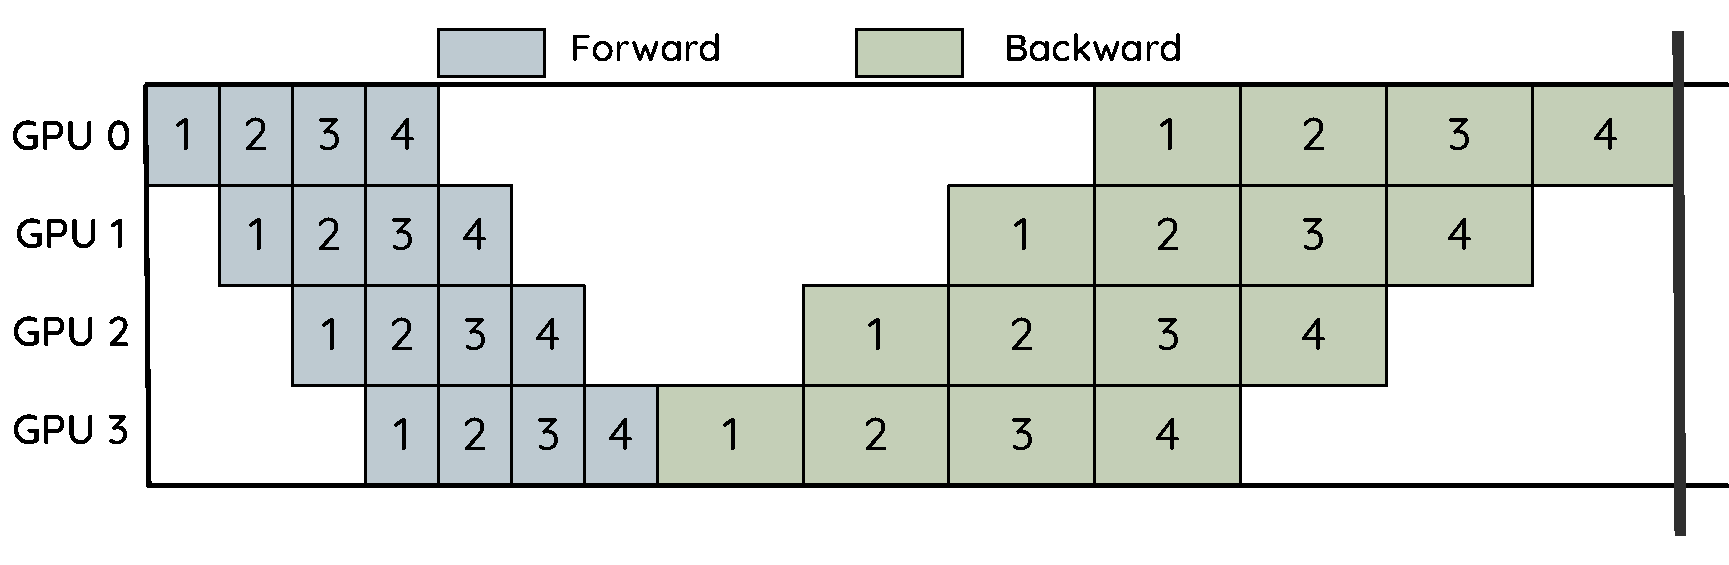
\includegraphics[width=0.95\linewidth]{GPipe-execution.pdf}
%   \caption{GPipe's Synchronous Pipeline Parallelism}
%   \label{fig:gpipe}
% \end{figure}
% \begin{figure}
%   \centering
%   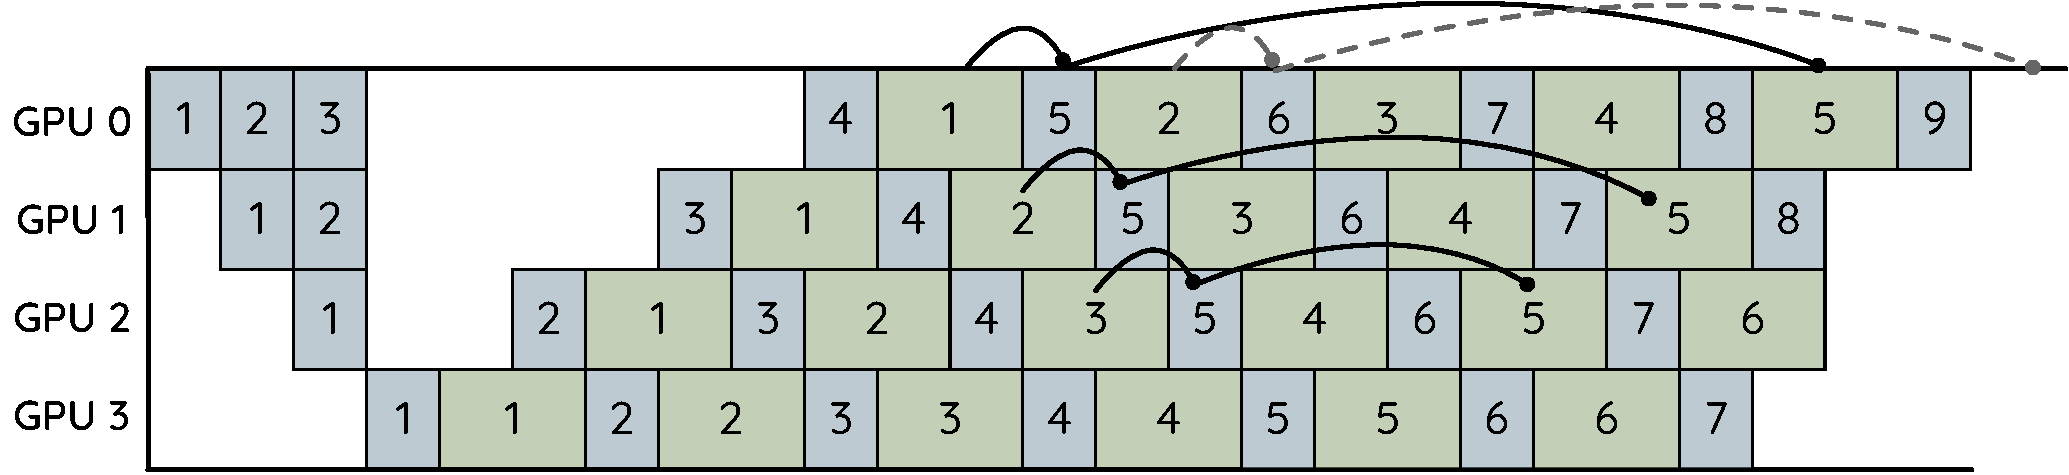
\includegraphics[width=0.95\linewidth]{PipeDream-execution.pdf}
%   \caption{PipeDream's Asynchronous Pipeline Parallelism}
%   \label{fig:pipedream}
% \end{figure}
\begin{figure}[htb]
  \centering
  % \hspace{-0.7cm}
  \subfigure[Synchornous Pipeline Parallel — GPipe]{
    \centering
    \label{subfig:gpipe}
    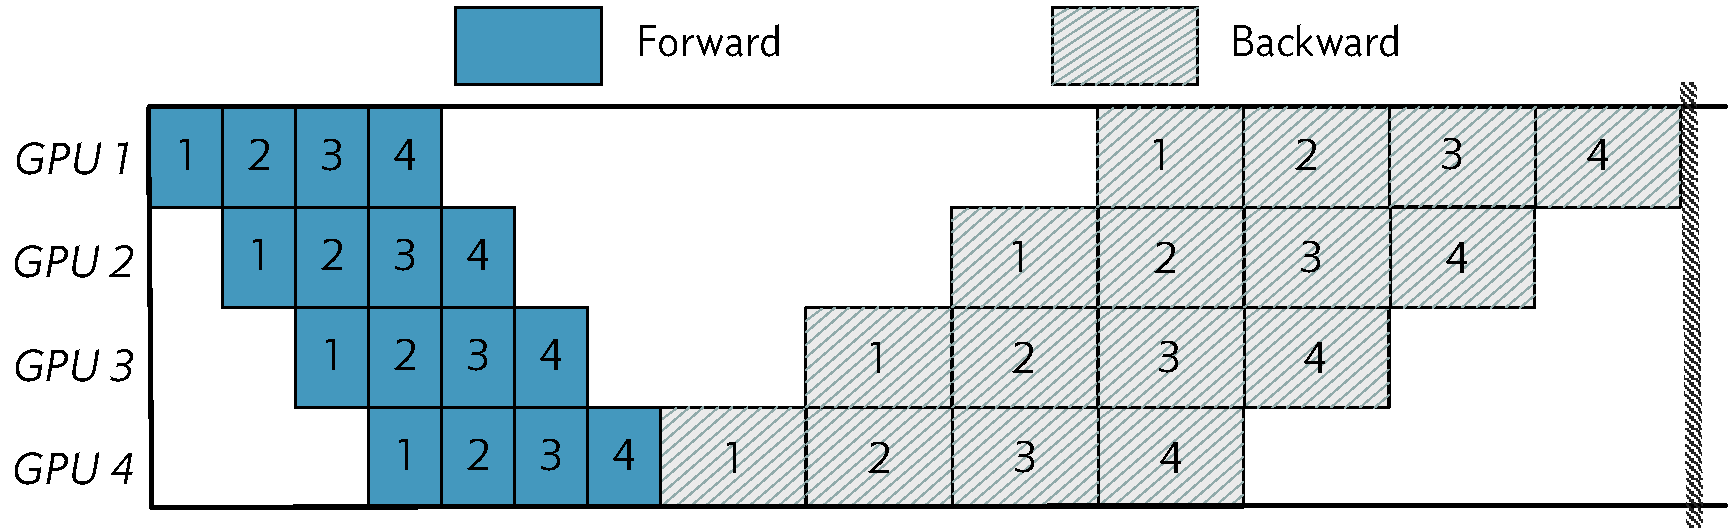
\includegraphics[width=1.0\linewidth]{GPipe-exec.pdf}
  }
  \subfigure[Asynchronous Pipeline Parallel — PipeDream]{
    \centering
    \label{subfig:pipedream}
    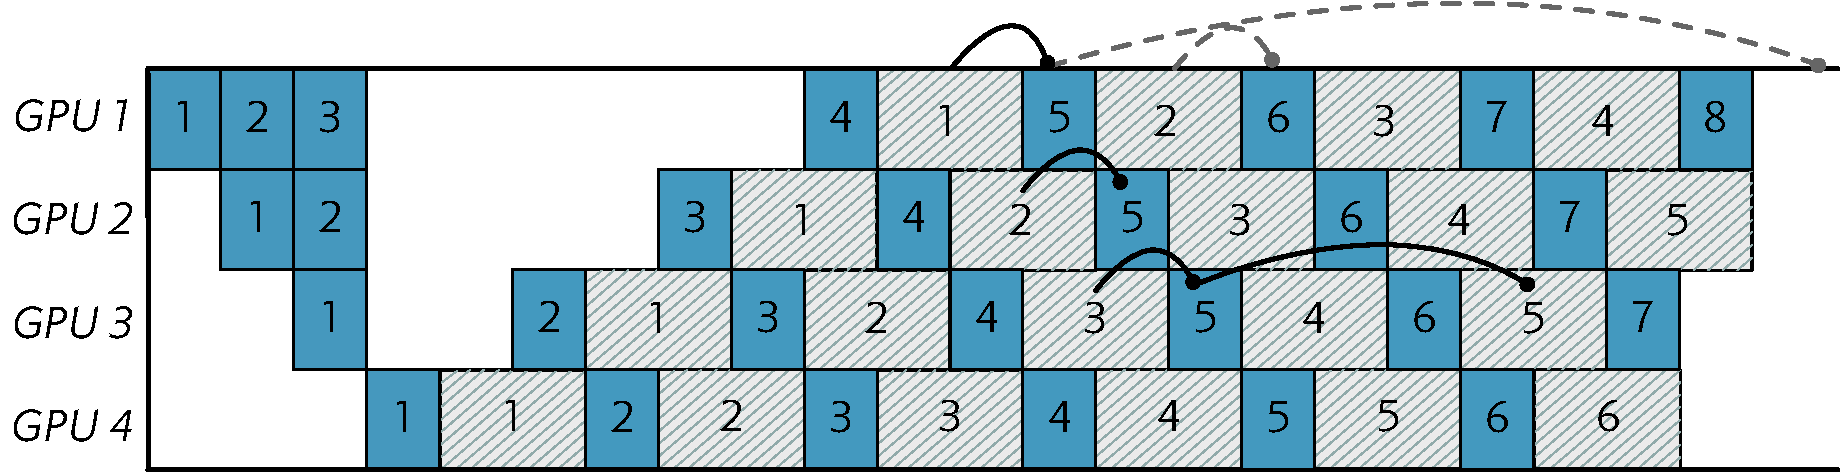
\includegraphics[width=1.0\linewidth]{PipeDream-exec.pdf}
  }
  \caption{Synchornous and Asynchronous Pipeline Parallel Execution}
  \label{fig:pp-exec}
\end{figure}

\subsection{Swap and Recomputation}
In previous works~\cite{vrhuVDNNVirtualizedDeep2016,chenTrainingDeepNets2016,wangSuperneuronsDynamicGPU2018,pengCapuchinTensorbasedGPU2020}
of memory optimization for DL training,
swap and recomputation (also named as \emph{activation checkpointing})
are already been proved to be two
effective approaches to reduce the memory footprint during the DNN's training.
Both \emph{swap} and \emph{recomputation} utilize the characteristic that
there is a time gap between two accesses to the same activation memory
in forward and backward propagation.
Swap aims to leverage the CPU memory as the external memory to extend the GPU memory limitation.
which copies the activation memory to CPU in forward pass
and copy back to GPU in backward pass, in which the vDNN~\cite{rhuVDNNVirtualizedDeep2016} is the pioneer.
Chen et al.~\cite{chenTrainingDeepNets2016} proposed the activation checkpointing technique to drop the
activation memory during forward propagation and perform the forward computation
again to regenerate the activation memory, which will incur about 30\% overhead to the overall training.
SuperNeurons~\cite{wangSuperneuronsDynamicGPU2018} and Capuchin~\cite{pengCapuchinTensorbasedGPU2020} proposes dynamic
swap and recomputation strategies to further reduce the memory footprint while maintaining training performance.
Wahib et al.~\cite{wahib2020scaling} added the swap memory optimization support in distributed training environment.
% TODO(hp): add related works for distributed environment
For pipeline parallelism,
GPipe~\cite{huangGpipeEfficientTraining2019} has integrated the recomputation mechanism.
vPipe~\cite{zhaoVPipeVirtualizedAcceleration2022} further propose a iterative pipeline partition algorithm
that considers \emph{swap, recomputation}, and \emph{partition} in conjunction.
AdaPipe~\cite{sunAdaPipeOptimizingPipeline2024} proposed a two-step dynamic programming algorithm
of pipeline partitioning and re-computation strategy for the 1F1B computation scheduling.
% However, these works perform model partitioning and memory optimization
% are all at a coarse granularity (layer block), which make it difficult to
% achieve both the memory and computation efficiency.
% Besides, they ignores the computation characteristics differences
% between the pipeline parallelism and single-GPU training,
% which cannot support efficient memory swap in pipeline parallelism.

% In recent years, the scale of deep neural networks has been growing increasingly large,
% especially in the field of natural language processing,
% such as large models like T5, GPT-4, and Huawei's PanGu.
% The memory capacity of a single GPU is no longer sufficient to accommodate such large-scale models,
% making the use of multiple GPUs for parallel training a common choice in both academia and industry.
% Among these parallel methods, data parallelism requires all GPUs to synchronize and update the entire
% model parameters in each iteration. As the model parameters grow larger, this communication overhead
% becomes increasingly significant. Tensor parallelism not only requires careful division of model operators
% but also necessitates synchronous communication between divided operators, which affects computational performance.
% Pipeline parallelism, in contrast to the two methods mentioned above, usually has much less communication volume
% because communication only occurs between adjacent stage GPUs, with the amount of communication being
% only the activation values and gradients at the division points.
% Moreover, this communication can be executed in parallel with computation,
% thus attracting extensive research and attention in the industry.
% However, due to the constraints of model division,
% pipeline parallelism often leads to a significant waste of GPU memory resources to ensure overall training performance,
% limiting the scale of the models it can support.


% %!TEX root = main.tex
\section{Observation}
\label{sec:observation}


%!TEX root = main.tex
% \section{Motivations and Opportunities}
\section{Challeges and Motivations}
\label{sec:cam}
\subsection{Memory Imbalance in Pipeline Parallelism}
Pipeline parallelism is designed to distribute large model training across multiple devices
when a single device's memory cannot accommodate it.
However, significant memory inefficiency arises due to imbalanced memory usage across pipeline stages,
which contradicts its intended purpose.
To highlight this imbalance,
we conducted a benchmark test on the peak memory usage of each stage in GPipe and PipeDream.
The test was performed on a server with 8 A100 GPUs (40 GB each),
with pipeline stages set to 4 and 8 for GPipe and PipeDream, respectively.
\begin{figure*}[t]
  \centering
  \begin{minipage}[t]{0.33\linewidth}
    \centering
    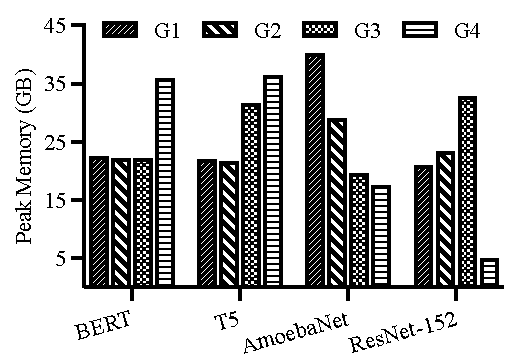
\includegraphics[width=0.95\linewidth]{GPipe-4GPUs.pdf}
    \caption{Peak Memory Usage of Each Stage on GPipe (4 GPUs)}
    \label{fig:gpipe-4gpus}
  \end{minipage}
  \begin{minipage}[t]{0.33\linewidth}
    \centering
    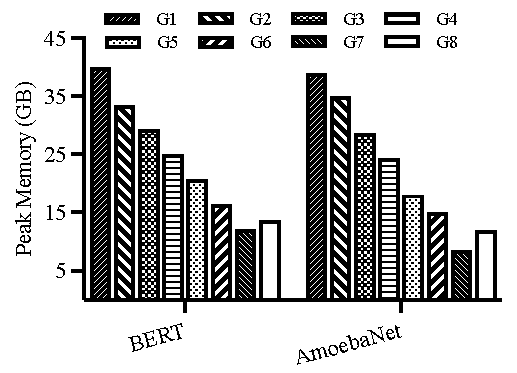
\includegraphics[width=0.95\linewidth]{PipeDream-8GPUs.pdf}
    \caption{Peak Memory Usage of Each Stage on PipeDream (8 GPUs)}
    \label{fig:pd-8gpus}
  \end{minipage}
  \begin{minipage}[t]{0.33\linewidth}
    \centering
    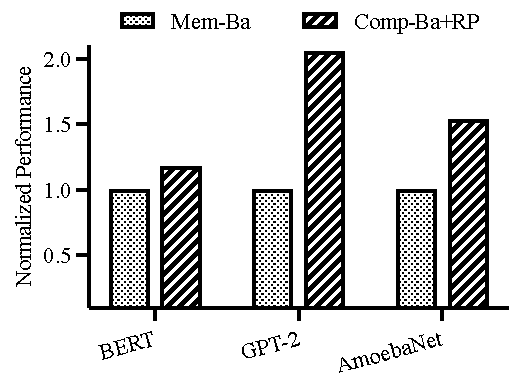
\includegraphics[width=0.95\linewidth]{normalized-perf.pdf}
    \caption{Normalized Performance of Two Different Partition Methods}
    \label{fig:norm-perf}
  \end{minipage}
\end{figure*}

Figure~\ref{fig:gpipe-4gpus} presents the benchmark results for GPipe, where G1 to G4 represent the GPU of different pipeline stages.
For the BERT model, the peak memory usage is nearly identical for the first three stages
but the last stage uses 13 GB more than the others.
This is because BERT, as a Transformer-based model with consistent computation and memory usage across its hidden layers,
shows balanced memory usage in the initial stages.
However, the last stage handles additional loss calculations and other post-processing functions,
leading to a significant memory spike.
A similar pattern is observed in T5, another Transformer-based model,
but with a peak memory shift to the third stage due to its encoder-decoder architecture.
In contrast, convolutional neural networks (CNNs) like ResNet-152 exhibit a different pattern.
Here, the ratio of computation times to memory usage varies with different types of layers.
For example, convolutional layers have longer computation times
while fully connected layers are more memory-intensive.
In ResNet-152, the last stage accounts for about 25\% of the total computation time but uses only 5 GB of memory,
creating a 27 GB difference compared to the third stage, which has the highest memory demand.
If peak memory usage across all stages is used as the baseline for GPU capacity,
this imbalance results in nearly 40\% and 34\% memory waste in ResNet-152 and AmoebaNet, respectively.

In synchronous pipeline parallelism,
memory imbalance across stages primarily arises from the uneven ratio
of computation time to memory usage among different layers in the model.
In asynchronous pipeline parallelism, this imbalance is further aggravated
by the varying number of copies of model parameters, activation memory, and gradients needed at each stage.
The benchmark result for PipeDream is shown in Figure~\ref{fig:pd-8gpus}.
The peak memory usage of the first stage reaches 40 GB,
while the smallest peak memory usage is only 12 GB in BERT.
In GPipe, the memory waste ratio for BERT is around 28\%, but in PipeDream, this waste ratio exceeds 40\%.
Furthermore, the memory waste ratio decreases by nearly 10\% compared to GPipe for AmoebaNet.
Whether using synchronous or asynchronous pipeline parallelism, significant GPU memory is wasted.
This memory waste limits the model size that can be accommodated to the stage with the highest memory usage,
despite substantial unused memory available on other GPUs.

\subsection{Computation Balance}
Based on the discussion above,
it is evident that focusing on balancing computation across pipeline stages
often leads to imbalanced memory usage, and vice versa.
Additionally, with memory optimization techniques like swapping and recomputation,
a key challenge arises when GPU memory is oversubscribed after partitioning a model for computational balance:
should the model be repartitioned to achieve more balanced memory usage,
or should memory optimization methods be applied to handle stages that exceed GPU capacity?
It’s difficult to determine which approach offers better training performance.
To explore this, we implemented two simple partitioning strategies in PipeDream for comparison.
The first method is memory-balanced partitioning (Mem-ba),
while the second combines compute-balanced partitioning with recomputation (Comp-ba+RP).
Both strategies achieve comparable maximum batch sizes,
and communication overhead does not significantly impact training performance.

The normalized performance results are shown in Figure~\ref{fig:norm-perf}.
Across all three models, the second method consistently outperforms the first,
particularly with the GPT-2 model,
where the training performance of Comp-Ba+RP is more than twice that of memory-balanced partitioning.
This performance gap is due to the significant difference in computation time between
the longest and shortest stages after memory-balanced partitioning in GPT-2.
Specifically, the computation time of the fourth stage reaches 286.275 ms
while the first stage only takes 29.104 ms — a nearly 10$\times$ difference.
As a result, the overall pipeline performance is severely constrained by the long computation time of the fourth stage.
Additionally, recomputation in GPT-2 provides significant memory savings with minimal additional computation overhead.
In the Comp-Ba+RP method, the total computation time for the fourth stage is reduced to 145.89 ms,
while the first stage, which requires more recomputation, increases to 136.89 ms.
This results in the fourth stage’s computation time being nearly halved compared to Mem-ba.
Similar improvements are observed in BERT and AmoebaNet, with performance gains of 1.18$\times$ and 1.54$\times$, respectively.
It is important to note that while the second method consistently outperforms in this benchmark,
this may not always hold true in every scenario.
The purpose of this section is to demonstrate that optimizing
pipeline parallel performance while considering memory limitations,
partitioning strategies, and memory optimization techniques is a complex and challenging problem.

\subsection{Motivation}
\label{sec:mot}
We observed that DL compilation techniques like XLA~\cite{sabneXlaCompilingMachine2020}
and TorchDynamo~\cite{anselPyTorchFasterMachine2024},
widely used in tensor parallelism for fine-grained analysis and automatic code generation,
have not been applied to pipeline parallelism in previous research.
Building on the fine-grained analysis provided by DL compilation,
we identified two key memory usage characteristics during model training that can guide pipeline partitioning.

First, most activation memory sizes are small,
making it easier to find low communication volumes between stages for efficient pipeline partitioning.
We profiled activation memory sizes for BERT, T5, GPT-2, and AmoebaNet, with results shown in Figure~\ref{fig:act-mem-cdf}.
In Transformer-based models, the largest activation memory is typically at the output layer,
which resides in the last stage and does not contribute to inter-stage communication.
For AmoebaNet, the largest activation memory (about 580 MB) comes from outputs of certain convolutional layers,
appearing only five times, so they are omitted in the figures. 
The data reveals that in GPT-2, T5, and AmoebaNet, over 90\% of computational nodes have activation memory sizes below 80 MB.
In T5, aside from the final output node, most activation memory is only around 50 MB.
In BERT, nodes with activation memory no greater than 128 MB account for over 80\% of the total nodes.
Even as batch size increases with pipeline partitioning, the communication overhead remains manageable.
For example, with four pipeline stages, a 4$\times$ transfer of 128 MB (512 MB total) over
a PCIe 3.0 $\times$16 link would take less than 40 ms, which is significantly shorter than the computation time.
\begin{figure}[htb]
  \centering
  \subfigure[Activation memory]{
    \centering
    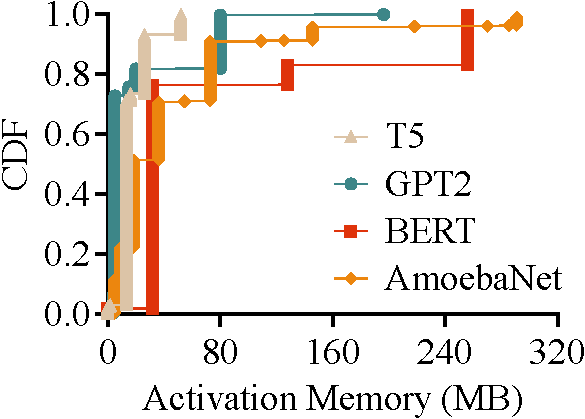
\includegraphics[width=0.47\linewidth]{act-mem-cdf-crop.pdf}
    \label{fig:act-mem-cdf}
  }
  \subfigure[Consumed Memory]{
    \centering
    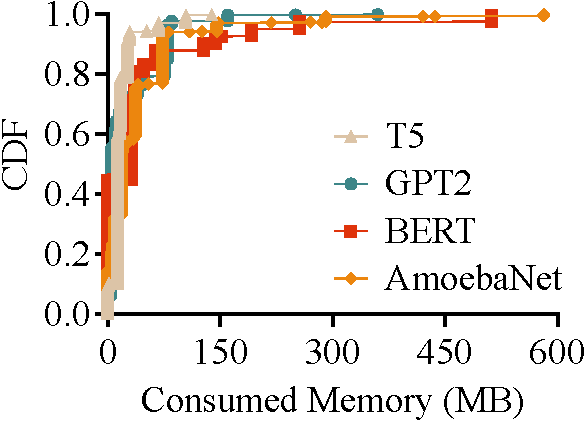
\includegraphics[width=0.47\linewidth]{consumed-mem-cdf-crop.pdf}
    \label{fig:cons-mem-cdf}
  }
  \caption{CDF of Node Activation Memory and Consumed Memory}
  \label{fig:mem-cdf}
\end{figure}

Secondly, the distribution of absolute memory consumption is shown in Figure~\ref{fig:cons-mem-cdf}.
Memory consumption here is calculated as the sum of memory allocated and released during node execution,
with released memory represented as a negative value.
The results show that in all four models, nearly 90\% of memory consumption per node is under 150 MB.
This suggests that partition points between stages can be flexibly adjusted between nodes with minimal memory usage,
allowing for small changes in the overall memory footprint of each stage while keeping communication overhead low.

Based on these insights, we propose a partitioning theorem for pipeline parallelism,
which will be discussed in detail in the next section.

%!TEX root = main.tex
\section{Design of DawnPiper}
\label{sec:design}
\subsection{Design Overview}
The overall architecture of DawnPiper is shown in Figure~\ref{fig:sys_arch},
which includes three modules for the partition of the pipeline parallelism.
We will give them a brief introduction next.

\begin{figure*}[t]
  \centering
  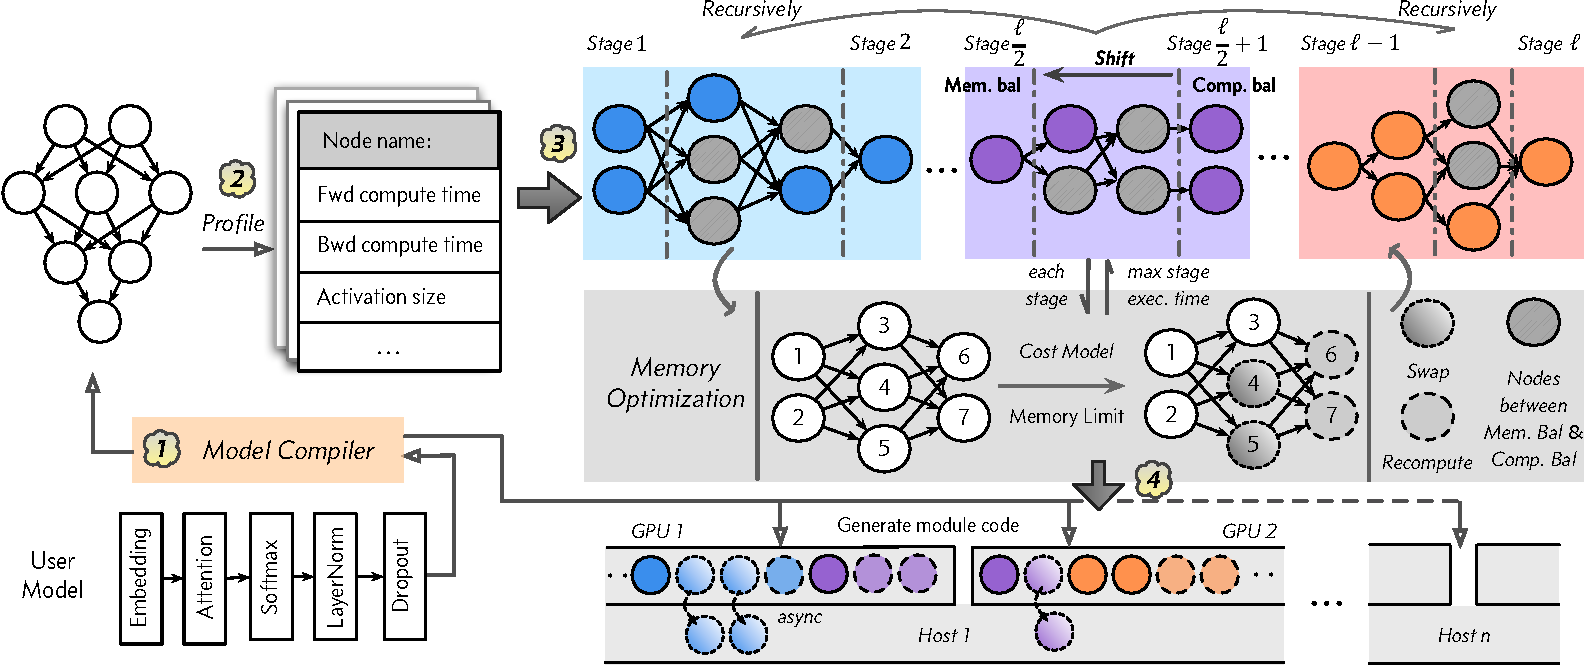
\includegraphics[width=0.95\linewidth]{pp-opt-arch-crop.pdf}
  \caption{DawnPiper System Architecture}
  \label{fig:sys_arch}
\end{figure*}

\textbf{Compiler:} Once the user submits a model for pipeline parallelism,
the \emph{compiler} obtains its fine-grained computation graph via DL compilation.
The computation graph includes all operators (nodes) in the training process and
the connection information between nodes.
This compilation-based approach allows subsequent model partitioning
and memory optimization to be performed
on this fine-grained computation graph.
In the meantime, the model code of each stage after the model partitioning
can be automatically generated based on the partitioned sub-graphs,
eliminating the need for manual involvement in the process,
making the system highly versatile and practical.

\textbf{Profiling:} This module is responsible for acquiring the
execution metadata of each node for the fine-grained computation graph.
For a node \emph{n}, its execution metadata data include the forward computation time $t_f^n$,
backward computation time $t_b^n$, the activation memory size $m_a^n$,
the size of the model parameters and optimizer states at this node $m_p^n$,
and the list of saved tensor ${st}^n$.
Based on the nodes dependencies information,
the memory size that needs to be released at each node can be inferred as $m_d^n$.
With the above information, the computation time, peak memory usage,
and inter-stage communication volume of each stage can
be easily deduced when partitioning the model at any nodes.
Meanwhile, the memory optimization policy could also be decided using the metadata.

\textbf{Pipeline Partitioning:} This module is responsible for the pipeline partition.
The basic idea is limiting the pipeline partition range between
the positions of the compute-balance and memory-balance.
When traversing each possible partition positions,
the memory optimization module will identifie the minimum
memory optimization cost that allows each stage's training process to
meet the GPU memory capacity limit for a given model partitioning.
After traversing all model partition positions,
the target partition strategy is the one with the
smallest time of the longest execution stage.

% \textbf{Memory Optimization Module:} This module identifies the minimum memory optimization cost method
% that allows the model execution process in each stage to meet the GPU memory capacity limit for each
% pipeline partitioning method obtained by traversing every partition position in the aforementioned
% pipeline partitioning module. This allows the deduction of the longest execution time stage under
% this partition strategy and records the corresponding execution time.

Next, we will dive into the details of the pipeline parallelism partition and memory optimization algorithms.

\subsection{Pipeline Terminology and Partition Theorem}
The number of the pipeline stages is denoted as $\ell$,
For a pipeline stage $x$, $x \in [1, \ell]$,
the set of computation nodes it contains is defined as $\mathcal{N}_x$.
The computation time of this stage can be obtained
by adding the forward and backward computation times
of all nodes in the set, as shown in Equation (3.1).
\begin{align}
  T_x=\sum_{n \in \mathcal{N}_x}\left(t_f^n+t_b^n\right)
\end{align}

The peak memory usage of a stage can be calculated according
to the set of nodes in the stage and the pipeline scheduling method.
The optimal performance partition is to make the
processing time of all stages as close as possible.
Since the inter-stage communication mentioned earlier
can be minimal and can be executed concurrently with computation,
the goal is to minimize the computation time of the longest stage,
i.e., the stage with the longest execution time, among all partitioning strategies,
while the peak GPU memory usage of all stages are less than the GPU memory capacity,
that is $minimize\ \max_{1 \leq x \leq \ell} T_x$.

Due to the fine-grained computation graph obtained by DL compilation,
the entire search space will grow exponentially and become very large
if we consider all possible partition positions coupled with each
possible memory optimization combinations.
Therefore, it is necessary to eliminate unreasonable
pipeline partitions to shrink the total search space.
We propose a partition theorem to restrict the partition space
by leveraging the memory usage features mentioned above.

\textbf{Theorem:} Given a model that needs to be divided into two pipeline stages,
the optimal pipeline partition must exist in the closed interval between the compute-balance and
memory-balance partition positions when the following three conditions are met:
1) The computation time and memory usage during the forward propagation
show a monotonically increasing trend as operations are continuously scheduled;
2) The time required for inter-stage communication is
always less than the computation time of the stage;
3) The memory optimization targets are evenly distributed throughout the entire model.

\textbf{Proof:} For convenience, let's illustrate with the simplest example of a
2-stage pipeline parallelism, and the proof can be extended to more than 2 stages accordingly.
The pipeline compute-balance and memory-balance partition positions
are denoted as $\rho_{cb}$ and $\rho_{mb}$, respectively.
For the 1F1B computation scheduling in the asynchronous pipeline,
since the earlier stages need to store more activations and parameters memory,
the position of $\rho_{cb}$ is usually further to the right than $\rho_{mb}$
(the case where the positions are reversed can also be proven using the following method).
As shown in the model partitioning in step 3 of Figure~\ref{fig:sys_arch},
if the partition position is moved further to the right from $\rho_{cb}$,
which means more computation nodes are assigned to the first stage,
due to the feature of monotonicity of computation time and memory usage,
and the negligible communication overhead,
the computation time and peak memory usage of the first stage are increasing,
while that of the second stage are decreasing.
Since the memory optimization targets are essentially
evenly distributed throughout the entire model structure,
there will not be a stage with smaller memory usage
that requires a greater memory optimization cost to meet the GPU memory limit.
This leads to the fact that no matter whether memory optimization is needed,
the first stage is definitely the longest stage,
and it exceeds the computation time of the longest stage under the compute-balance partition.
So the pipeline parallel training performance is continuously
decreasing as the partition position moves from $\rho_{cb}$ to the right.
Similarly, if the partition position is moved further to the left from $\rho_{mb}$,
then the second stage is definitely the longest computation time stage,
and it will continuously increase as the movement progress.

\subsection{Compute and Memory Balance Partition}
In this section, we will introduce how to find the compute-balance and memory-balance partition positions.
The basic process is to traverse the nodes in the compute graph according to the execution order,
continuously accumulating the forward/backward computation time or the memory consumption.
Since the memory footprint of each stage needs to consider the
stage number in asynchronous pipeline parallelism,
while the computaiton time of each stage can be simply added,
we only give the memory-balance partition algorithm for PipeDream
in this section which is shown as Algorithm~\ref{alg:mem-ba}.

Before the algorithm begins,
we first traverse the compute graph to calculate the depth of each node.
Nodes with the same depth are sorted by the start time of forward computation,
and this node set is denoted as $\mathcal{N}_\mathcal{G}$ for the algorithm input.
Besides, the inputs also include the GPU peak memory usage $M_\mathcal{G}$ and the number of pipeline stages $\ell$.
The output of the algorithm is the partition positions of each stage $\rho_x$.
The ratio of activations and parameters copies that need to be stored from the first stage
to the last stage is $\ell:(\ell-1):(\ell-2):\cdots:1$ in PipeDream.
If the peak memory usage corresponding to each stage for a micro-batch is defined as $M_x$,
in order to make the peak memory usage of all stages equal,
the following equation must exist:
\begin{align}
  \ell \times M_1=\cdots=(\ell-x+1) \times M_x=\cdots=M_{\ell}
\end{align}
% \ell \times M_1=(\ell-1) \times M_2=\cdots=(\ell-x+1) \times M_x=\cdots=M_{\ell}
Based on this equation, the $M_x$ of each stage can be calculated,
as shown in lines 2-5 and line 12 of Algorithm~\ref{alg:mem-ba}.
In this way, the algorithm can continuously traverse the nodes,
first adding the activation memory, parameter memory, and optimizer state memory size of the node,
and then determining whether it exceeds the previously recorded peak memory size.
Next, subtract the memory size that needs to be released at this node,
and continue to repeat until the peak memory size reaches the current stage's $M_x$.
At this point, current node is the position where this stage needs to be partitioned.
It should be noted that for the sake of convenience in description,
the partition position is a single node,
but it is usually a set of nodes in practice.

\begin{algorithm}
  \SetKwInOut{Input}{Input}
  \SetKwInOut{Output}{Output}
  $x \leftarrow 1,cur\_mem \leftarrow 0,peak\_mem \leftarrow 0$\;
  \For{$i$ in $[0,\ell)$}
  {
    $sum += \ell \div (\ell-i)$\;
  }
  $M_x \leftarrow M_\mathcal{G} \div sum$\;
  \For{$n$ in $N_\mathcal{G}$}
  {
    $cur\_mem += m_a^n + n_p^n$\;
    $peak\_mem \leftarrow \max(cur\_mem,peak\_mem)$\;
    $cur\_mem -= m_d^n$\;
    \If{$peak\_mem \ge M_x$}
    {
      $\rho_x \leftarrow n,x \leftarrow x + 1$\;
      $M_x \leftarrow (\ell \div (\ell -x + 1) \times M_1)$\;
      $cur\_mem, peak\_mem \leftarrow 0$\;
      \If{$x == \ell$}
      {
        \textbf{break}\;
      }
    }
  }
\caption{Memory balance partition in PipeDream}
\label{alg:mem-ba}
\end{algorithm}

\subsection{Binary Pipeline Parallel Partition}
If the peak memory footprint of all stages at compute-balance partition
are less than the GPU memory capacity,
then this is already the optimal pipeline partitioning
in terms of performance.
Otherwise, it is necessary to continuously move the partition position from
$\rho_{cb}$ the towards the $\rho_{mb}$ or take memory optimization
operations to reduce memory usage.
Both of these two methods will change the execution time of a stage,
it is difficult to analyze which partition and memory optimization strategy
will produce the optimal pipeline parallel performance.
Therefore, it is necessary to perform a combination traversal of the possibilities.
During the process, given a pipeline partition, the goal of memory optimization for each stage
is to minimize the memory optimization cost while meeting the GPU memory capacity limit.
Define the minimum memory optimization cost time corresponding to stage $x$ as $T_x^{moo}$,
then the objective of the pipeline partition with memory optimization
is to $minimize\ \max_{1 \leq x \leq \ell} (T_x + T_x^{moo})$ .

It should be noted that during the process of moving from the $\rho_{cb}$
to the $\rho_{mb}$, if the peak memory usage of the adjacent two stages after partitioning
are less than the GPU memory limit without memory optimization,
then there is no need to continue to traverse subsequent partition possibilities.
This conclusion can also be proven using the above theorem.
In simple terms, if the partition position continues to move at this time,
the computation time and memory usage of the stage
with more computation time will continue to increase.
Regardless of whether it still needs memory optimization,
its total computation time will continuously increase
and exceed the longest execution stage's computation time at the current partition position.
% Therefore, the shortest time of the longest execution stage during the partition position movement
% will definitely not appear behind this partition position.

Based on the above discussion,
the naive idea is to start from the $\rho_{cb}$
of the first stage and continuously move towards the $\rho_{mb}$ for traversal.
For each position, calculate the $\rho_{cb}$ and
$\rho_{mb}$ of the subsequent $\ell - 1$ stages
until the last two adjacent stages.
Then we use memory optimization to obtain the minimal cost for each stage.
By that, we can know the computation time of the longest execution stage for the current partition positions.
After traversing all partition positions,
we can find the optimal partition and memory optimization strategy.
% is the strategy corresponding to the minimum computation time of the longest execution stage.
Although the range of each partitioning operation is restricted between the $\rho_{cb}$
and the $\rho_{mb}$, the search space increases exponentially with the number of pipeline stages.
Therefore, to cope with the pipeline parallel partitioning of longer stages,
we adopts a binary pipeline parallel partitioning method,
which first enumerates from the middle stage of the pipeline.
Each time the middle is divided, the left and right parts are regarded as two stages
to achieve compute-balance and memory-balance.
In this way, the shortest computation time of the longest execution stage
on the left and right parts at each binary partitioning can be found level by level.
When the outermost level finishes traversing all possible partition positions,
then the optimal partition strategy can be found.
By that, the complexity of the partition algorithm is successfully
reduced to $\mathcal{O}(\varphi^{log\ell})$,
where $\varphi$ represents the number of possible partitions that
need to be traversed from the $\rho_{cb}$ to the $\rho_{mb}$.
This number is far smaller than the total number of nodes in the model.
Take the BERT for example, its total nodes are more than 1000,
in which the number of nodes in this range are less than 100.
% and the communication optimization method to be introduced below can further reduce the
% possible partition positions.
The overall process of this partitioning method is shown in Algorithm~\ref{alg:binary-partition}.

\begin{algorithm}[t]
  \SetKwInOut{Input}{Input}
  \SetKwInOut{Output}{Output}
  \SetKwFunction{Fmain}{BinaryPartition}
  \SetKwFunction{Fadj}{AdjacentPartition}
  \SetKwProg{Fn}{Function}{:}{}
  \Fn{\Fadj{$\mathcal{N},sid$}}
  {
    $\rho_{cb},\rho_{mb} \leftarrow CompMemBalPartition(\mathcal{N}, sid, \ell)$\;
    \If{$\max_{sid \le x \le sid+1} ((\ell-x+1) \times M_x^{\rho_{cb}}) < M$}
    {
      \textbf{return} $\max_{sid \le x \le sid+1} T_x^{\rho_{cb}}$\;
    }
    $sorted\_pps \leftarrow IdentifyAndSort(\rho_{cb},\rho_{mb})$\;
    \For{$\rho \leftarrow sorted\_pps$}
    {
      $mopt_l,min\_t_l \leftarrow MemOpt(\mathcal{N}_{sid},M)$\;
      $mopt_r,min\_t_r \leftarrow MemOpt(\mathcal{N}_{sid+1},M)$\;
      $mopt \leftarrow mopt_l \cup mopt_r$\;
      $par\_dict[\rho] \leftarrow (\max(min\_t_l,min\_t_r),mopt)$\;
      \If{$!mopt$}
      {
        \textbf{break}\;
      }
    }
    \textbf{return} $\min(par\_dict)$
  }
  
  \Fn{\Fmain{$\mathcal{N},\mathcal{L},\mathcal{R}$}}
  {
    \If{$\mathcal{R}-\mathcal{L}==1$}
    {
      \textbf{return} $AdjacentPartition(\mathcal{N},\mathcal{L})$\;
    }
    $mid \leftarrow (\mathcal{L}+\mathcal{R}) /div 2$\;
    $\rho_{cb},\rho_{mb} \leftarrow CompMemBalPartition(\mathcal{N}, mid, \ell)$\;
    \For{$\rho \leftarrow sorted\_pps$}
    {
      $\rho_l,mopt_l,min\_t_l \leftarrow BinaryPartition(\mathcal{N}_{\mathcal{L}},\mathcal{L},mid)$\;
      $\rho_r,mopt_r,min\_t_r \leftarrow BinaryPartition(\mathcal{N}_{\mathcal{R}},mid+1,\mathcal{R})$\;
      $mopt \leftarrow mopt_l \cup mopt_r$\;
      $par\_dict[\rho] \leftarrow (\max(min\_t_l,min\_t_r),mopt)$\;
      \If{$!mopt$}
      {
        \textbf{break}\;
      }
    }
  }

\caption{Binary pipeline parallel partition}
\label{alg:binary-partition}
\end{algorithm}

The \texttt{AdjacentPartition} function of the Algorithm~\ref{alg:binary-partition}
describe how to find the partitioning and memory optimization strategy
that minimizes the difference in computation time between two adjacent stages.
The $\rho_{cb}$ and $\rho_{mb}$ of two adjacent stages
can be easily found by modifying Algorithm~\ref{alg:mem-ba}.
The line 7-8 describes the memory optimization process for the adjacent stages which
finds the policy that can achieve the shortest execution time under the memory limit.
The line 10-13 means the traversal process can exit in advance
when there is no memory optimization for the two stages.
This function finally returns the optimal partition and memory optimization strategies
and the corresponding execution time of the longer stage.
The \texttt{BinaryPartition} function of the Algorithm~\ref{alg:binary-partition}
is the main process of the binary partitioning algorithm.
The line 18-19 invokes the above \texttt{AdjacentPartition} function
when reaching two adjacent stages.
Otherwise, it calculates the $\rho_{cb}$ and $\rho_{mb}$ when partitioning from the middle.
The lines 24-25 represent the optimal results of the left and right partitions that continue to be
recursively divided, including the partition position, memory optimization strategy,
and the shortest execution time of the longest stage.
In this way, the final optimal pipeline partitioning and memory optimization strategy
can by obtained by calling \texttt{BinaryPartition}$(\mathcal{N}_\mathcal{G}, 1, \ell)$.

Note that although the above algorithm requires that the number of pipeline stages
need to be an exponential number of 2,
we will traverse from the first stage's compute/memory-balance partition positions
when the left number of pipeline stages is 3.
Hence, the proposed algorithm can handle any number of pipeline stages.
% $BinaryPartition(\mathcal{N}_\mathcal{G}, 1, \ell)$.
% the final optimal pipeline partitioning and memory optimization strategy results can be obtained.

\textbf{Communication Optimization:} It should be noted that a premis
of the partitioning theorem is that the communication overhead
will not become a factor affecting the efficiency of pipeline parallelism.
Therefore, it is necessary to avoid partition positions
that will generate large communication volumes
during the traversal process within the partition range.
As mentioned in Section~\ref{sec:mot}, there are a large number of computation nodes 
and the majority of their activations memory are very small.
Firstly, we can determine the inevitable memory communication,
i.e., a node owns an edge that is very far from the partition range,
which means that no matter how the partition strategy within this range is adjusted,
the data transmission of this node's activation value is inevitable,
such as the output of the initial embedding layer in BERT.
Such memory communication can be ignored.
For the remaining nodes, we will illustrate how to find a partition position
with a smaller communication overhead via a simple example.
Suppose there is a partition in which the activations of three nodes with the same depth
need to transmitted to the next stage.
Then we can find the lowest common leaf node of these nodes.
If this node is the only edge they are connected to,
then the partition that requires the transmission of multiple nodes' activation
can be optimized to only need to transmit the activation of a single node.
Meanwhile, such leaf node are usually very close to find,
which means the impact on the computation time and memory footprint
of the adjacent two stages is relatively small.

\subsection{Memory Optimization}
The goal of memory optimization is to minimize the execution time
of the stage while meeting the GPU memory limit for a given partitioning.
This objective is very similar to memory optimization in single-GPU training.
Therefore, we utilize the cost model in Capuchin~\cite{pengCapuchinTensorbasedGPU2020}.
In short, this model use \emph{FreeTime} and \emph{Memory Saving Per Second (MSPS)}
for evaluating the memory swapping and recomputation, respectively.
It first choose memory swapping until there is no computation
to overlap the data transfer.
Then the smaller performance overhead method between the memory swapping
and recomputation will be adopted.
In DawnPiper, we can easily obtain the memory optimization candidates through
the saved tensors list of each node's metadata.
Moreover, the \emph{FreeTime} and \emph{MSPS} of a candidate
can also be calculated via the node's metadata.

Nonetheless, there are some differences in terms of memory swapping in pipeline parallelism.
Firstly, multiple GPUs typically share the same host memory in pipeline parallelism.
Therefore, the CPU memory is not an unlimited resources under such circumstances.
For example, a 8 A100 GPUs server in which each stage swaps 40 GB memory,
resulting in a total of 320 GB of CPU memory requirement.
Moreover, such CPU memory needs to be page-locked
for ensuring the asynchrony of memory swapping,
which further increases the scarcity of this resource.
Therefore, we limit the memory swapping size to one-fourth
of the total host memory size by experience.
Secondly, a memory swap in a micro-batch means that
the same memory will be swapped multiple times
in mainstream 1F1B scheduling pipeline parallelism.

% Although the interval between memory swapping out and swapping in in the earlier stages is not only the inter-layer computation
% in single-GPU training but also the computation of different micro-batches, for inputs with the same micro-batch number,
% its memory swapping in cannot be performed before the start of its backward computation,
% as this would cause a memory shortage in the forward computation of other micro-batches.
% This means that the computation time available for overlapping data transfer in memory swapping is consistent
% in pipeline parallel training and single-GPU training.
% The assessment of recomputation benefits is unified in these two training modes, that is,
% to exchange less recomputation time for greater memory occupation reduction.
% Therefore, this section uses the memory optimization method in single-GPU training to
% find the minimum cost memory optimization strategy for each stage in pipeline parallelism that meets the memory limit.
% This method only needs to traverse the nodes once, as shown in Algorithm 3.3.
% First, line 1 calculates the amount of memory that needs to be saved for the current stage $x$.
% Secondly, recomputation uses the amount of memory that can be saved per second in single-GPU memory optimization
% to assess the benefits of recomputation for each node, that is, for each node after model compilation,
% calculate their ${MSPS}_n = \frac{m_a^n}{t_f^n}$, the larger the MSPS means the greater the recomputation benefit.
% Memory swapping uses the memory swapping idle time to assess its benefits.
% In this way, through the list of tensors saved for each node in the model test and analysis,
% all node output activation values that need to be saved during the backward computation process can be obtained,
% and then they can be sorted according to the above benefit estimation formula, as shown in line 2.
% Then, for each candidate memory optimization object, calculate their memory optimization cost and recomputation cost.
% If the current memory size of memory swapping has exceeded the preset threshold, then recomputation will be performed at this time.
% When the total amount of memory for memory optimization reaches the amount of memory that needs to be saved, exit,
% so as to obtain the strategy of minimum memory optimization cost under the memory limit.


%!TEX root = main.tex
\section{Implementation}
\label{sec:imp}
In this section, we will introduce how to compile and then profile a model in PyTorch.
Meanwhile, we also introduce the implementation of the memory swapping and recomputation.
Although the implementations are customized to the PyTorch framework,
the overall method of this paper is applicable for other DL frameworks, such as TensorFlow~\cite{abadiTensorFlowSystemLargeScale2016}.

\subsection{Compilation and Profiling}
\textbf{Compilation:} The essence of model compilation in this paper is
to obtain its fine-grained computation graph,
which can expanding the model partitioning and memory optimization space
while facilitating the automatic generation of each pipeline stage's module code.
It does not require the internal splitting and
tracking of an operator as in tensor parallelism.
Therefore, we utilize the \texttt{torch.fx}~\cite{reedTorchFxPractical2022}
provided by the official PyTorch to transform the model provided by the user scripts.
The \texttt{torch.fx} library is a pure Python system for
capturing and transforming the neural network structure in PyTorch through tracing.
It does not break down and trace the internal computations of nn.Module operators.
Users can freely modify the captured computation graph,
and torch.fx can generate corresponding Python code based on the modified computation graph.

\textbf{Profiling}: Regarding profiling the forward and backward
computation time of nodes after compilation,
we inserts timing hook functions to the start and the end of the corresponding computations.
The first few training iterations during warmup phase are excluded,
and then calculate the average value of 50 batches of stable iterations.
As for obtaining the memory size of activations, parameters, and optimizer states,
a proxy input tensors with the same size are passed to the computation graph
and executing the graph once.
During this process, the corresponding memory sizes can be obtained
from the result tensors once a node's computation is finished.
Meanwhile, the saved tensor information of a node
can also be got from this graph running process.
Specifically, we achieve this through registering the hook function
\texttt{torch.autograd.graph.saved\_tensors\_hooks} provided by PyTorch to each node.

\subsection{Swap and Recomputation}
\textbf{Memory swap:} The PyTorch does not support memory swapping operations currently.
Although a tensor can be copied to the target device through
a simple \texttt{Tensor.to(device)} interface,
the underlying GPU memory of the tensor cannot be released
without deleting the tensor object when the data transfer is completed.
Therefore, we modifies the underlying source code of the tensor data structure in PyTorch,
through adding two functions that can directly release the underlying
GPU memory without deleting the tensor object,
and set the underlying memory address to the address provided by the parameter.
This allows for the release of underlying memory after memory swapping out,
and the setting of the original tensor's memory address to
the address of the swapped-in tensor.
As for when to trigger memory swapping operations,
we uses the hook registration function in PyTorch to insert
the memory operations to the corresponding position.
This step is before the model training,
and then the memory swapping operations will always be carried out
according to this strategy during the pipeline parallel training.

\textbf{Recomputation:} PyTorch provides
the \texttt{torch.utils.checkpoint} library for recomputation.
It is implemented by rewriting the parts of the module code that need recomputation.
It initializes the recomputation process when the corresponding backward computation just begins,
which can also be called as on-demand recomputation.
Since we do not need another GPU stream for early recomputation process,
the functionality provided by this library is sufficient enough.
In the meantime,
the module codes for the recomputation of each stage are
also automatically generated during the module code generation phase.


%!TEX root = main.tex
\section{Evaluation}
\label{sec:evaluation}
\subsection{Experimental setup}
\textbf{Server.}
We conducted the experiments on the server which is
equipped with 8 NVIDIA Tesla A100 GPUs, each with 40 GB of memory, PCIe 4.0 $\times$16,
an AMD EPYC 7402 2.8 GHz 24-core processor, and 504 GB of memory.
The server is installed with CentOS 7, the CUDA Toolkit 11.2 and cuDNN 8.4.1,
with PyTorch version 1.11, and Huggingface Transformers~\cite{wolf2020transformers} version 4.27.2. The NCCL library version is 2.10.3.

\textbf{Workloads.}
% \subsubsection{Workloads}
We conduct the evaluation on four state-of-the-art deep learning models, including:
BERT~\cite{devlinBERTPretrainingDeep2019}, GPT-2~\cite{radfordLanguageModelsAre2019}, T5 (Text-to-Text Transfer Transformer)~\cite{raffelExploringLimitsTransfer2020}, and AmoebaNet~\cite{realRegularizedEvolutionImage2019}.
BERT is proposed by Google AI Language which contains 1024 hidden layers and approximately 340 million parameters.
GPT-2 is a famous pre-trained model proposed by OpenAI,
which has achieved remarkable success in various NLP tasks.
We uses the large version in the evaluation which contains about 770 million parameters.
T5 is a sequence-to-sequence model proposed by Google.
We uses its large version which contains about 780 million parameters.
AmoebaNet is a neural network that is automatically generated by the Neural Architecture Search (NAS) algorithm,
which contains about 28 million parameters
% evolutionary strategy based on the genetic algorithm in neural network architecture search,
BERT and GPT-2 are both trained with the WikiText-103~\cite{merityPointerSentinelMixture2017} dataset and T5 uses the WMT-16~\cite{bojarFindings2016Conference2016} dataset.
These three models are trained with \emph{Adam} optimizer.
The AmoebaNet model is trained with the ImageNet~\cite{dengImagenetLargeScaleHierarchical2009} dataset and the stochastic gradient descent (SGD) optimizer.
Two configurations with pipeline stage numbers of 4 and 8 are tested.

\textbf{Baselines.}
We have set up four baselines to evaluate the memory efficiency and training performance, which are listed below.
% The memory efficiency is represented by the maximum trainable batch size
% Since there is no clear interval between the computation of two batches in asynchronous training
% as in synchronous training, it is not possible to compare the batch sizes equally between synchronous
% and asynchronous training. Therefore, this chapter compares the batch sizes separately when comparing them,
% and their detailed introductions are as follows.
\begin{itemize}
  \item ZeRO~\cite{rajbhandariZeROMemoryOptimizations2020}: It is developed by Microsoft to eliminate redundant storage related to parameters
  across GPUs in data parallel training.
  We select the optimization levels two and three, namely ZeRO-2 and ZeRO-3, in this evaluation.
  \item GPipe~\cite{huangGpipeEfficientTraining2019}: Since the original GPipe is implemented based on the Lingvo~\cite{shen2019lingvo} framework,
  we use torchgpipe~\cite{kimTorchgpipeOntheflyPipeline2020} instead for evaluation which is an re-implementation of GPipe on PyTorch.
  \item PipeDream~\cite{narayananPipeDreamGeneralizedPipeline2019}: It firstly profiles the model in runtime and then uses dynamic programming
  to make the longest computation time among all stages as small as possible.
  % It is an asynchronous pipeline parallel method proposed by Narayanan et al,
  % which adopts a 1F1B computation scheduling method in each stage to eliminate pipeline bubbles.
  % PipeDream first measures and analyzes the model to obtain the execution characteristics of the model,
  % and then uses dynamic programming to make the longest computation time in all divided stages
  % after division as small as possible. The open-source implementation of PipeDream is based on PyTorch.
  \item vPipe~\cite{zhaoVPipeVirtualizedAcceleration2022}: It is implemented based on the runtime of PipeDream.
  However, its partition algorithm is not open-sourced yet.
  By that, we have implemented the algorithm according to the description in the corresponding paper of vPipe.
  % It is a pipeline division method that comprehensively considers model division,
  % memory exchange, and re-computation, proposed by Zhao et al.
  % It adopts an iterative algorithm to dynamically find a balance between model division and memory optimization.
  % It is implemented based on the runtime system of PipeDream.
  % Since the division algorithm of vPipe is not open-sourced,
  % this chapter implements the corresponding model division algorithm in PipeDream
  % based on the algorithm description in the corresponding paper of vPipe.
  % In this section, vPipe-S is used to represent the synchronous pipeline parallel model of vPipe,
  % and vPipe-AS is used to represent the asynchronous pipeline of vPipe.
\end{itemize}

\subsection{Memory Using Efficiency}
In this section, we evaluate the maximum trainable batch size of each method
to reflect the GPU memory usage efficiency.
We use the micro batch size to compare in asynchronous pipeline parallel training
since it is not like synchronous training which has a
clear interval between the computation of two batches.
% Since there is no clear interval between the computation of two batches in asynchronous training
% as in synchronous training, it is not possible to compare the batch sizes equally between synchronous
% and asynchronous training. Therefore, we compares the batch sizes separately when comparing them,

% Since some methods use memory optimization techniques such as memory swapping and
% re-computation to increase the trainable batch size, such as GPipe and vPipe,
% and to compare the increase in batch size brought by different methods,
% we will compare methods without memory optimization with those that use memory optimization.

\subsubsection{Synchronous Pipeline Parallel Training}
We firstly perform the evaluation in the synchronous pipeline parallel training mode.
The number of micro-batches is equal to the pipeline stages in this experiment.
% First, a comparison of each method under the synchronous training model is made.
% In this mode, the batch size is equal to the micro-batch size multiplied by the number of splits.
% In this experiment, the number of splits is set to the number of pipeline stages.
The results are shown in Table~\ref{table:maxbs-sync},
and the synchronous training mode of vPipe and DawnPiper
are denoted as vPipe-S and DPiper-S, respectively.

It can be seen that ZeRO-2 and ZeRO-3 can achieve basically
the same maximum batch size on the four models,
and the maximum batch sizes of ZeRO-3 are even smaller on the T5 and AmoebaNet models.
This is because the extra memory space of memory optimization on model parameters of ZeRO-3
as the batch size increases,
the optimization of ZeRO-3 for the memory occupation of model parameters is no longer
sufficient to support a larger batch,
and it also requires additional memory buffers for communication.
For the results of GPipe and vPipe, it can be seen that the maximum batch sizes are basically
consistent with ZeRO on BERT, GPT-2, and T5.
% the maximum trainable batch size is basically consistent with the data parallel method optimized by ZeRO.
However, the batch sizes are much smaller than ZeRO on the AmoebaNet model.
This is because the Transformer-based models where the computation
and memory occupation of each layer are basically proportional,
making the division method of GPipe and vPipe,
which aims at balancing the computation time among stages,
also able to make the memory footprint of each stage basically balanced.
% However, on the AmoebaNet model, this batch size is much smaller than ZeRO,
% which is due to the Transformer-based models where the computation and memory occupation of each layer
% are basically proportional, making the division method of GPipe and vPipe-S, which aims at balancing
% the computation time between stages, also able to make the memory occupation between stages more balanced.
The situation is different on CNN models, where the computation
and memory occupation of layers are usually not proportional, that is,
a layer may have a long computation time but its memory usage may be very small,
such as the convolutional layer, which leads to a very uneven memory footprint
when trying to balance the computation time of each stage.
% under the condition of balanced computation time in each stage.
% AmoebaNet is a CNN model, where the computation and memory occupation of layers are not proportional, that is,
% a layer may have a long computation time but its memory occupation may be very small,
% such as the convolutional layer, which leads to a very uneven memory occupation under the condition
% of balanced computation time in each stage.
As a result, the maximum batch size that GPipe and vPipe can achieve
on the AmoebaNet model is 68\% and 46\% of ZeRO when the number of pipeline stages is 4.
This ratio becomes even smaller, only 58\% and 32\% as the number of pipeline stages increases to 8.
% Therefore, when the number of pipeline stages is 4,
% the maximum batch size that GPipe and vPipe-S can achieve on the AmoebaNet model is 68\% and 46\% of ZeRO, respectively.
% When the number of pipelines increases to 8, this ratio becomes even smaller, only 58\% and 32\%.
In the meantime, it is noted that GPipe can achieve a larger batch size compared to vPipe,
while the results are reversed after enabling memory optimization.
It is because the stage of the memory bottleneck becomes different when enabling memory optimization.
% because after enabling memory optimization,
% the stages that become the memory bottleneck in GPipe and vPipe-S are different.

DawnPiper achieves the largest batch size among all methods on the BERT, GPT-2, and T5.
Without memory optimization, it can increase the batch size by up to 1.2$\times$ and 1.55$\times$
compared to the second best method, vPipe, when the pipeline stages are 4 and 8, respectively.
% when there is no memory optimization.
% Without enabling memory optimization, it can increase the batch size by up to 1.2$\times$ and 1.55$\times$
% compared to the next best method, vPipe-S, when the pipeline stage is 4 and 8, respectively.
Note that the maximum batch sizes are consistent across all methods for GPT-2
due to its significant memory footprint during training.
Even a slight increase in batch size results in a notable increase in memory usage.
% the memory footprint during the training is significantly large.
Although DawnPiper can refine the pipeline partition space,
it cannot further increase the batch size.
% It should be noted that for the GPT-2 model, the maximum batch size is the same across all methods.
% This is because its model training memory occupation is very large, and due to its model structure characteristics,
% the memory occupation of each stage is also quite similar when evenly divided by computation.
% Although DawnPiper-S can refine the model division space,
% it cannot further increase the batch size.
For AmoebaNet, the maximum batch size of DawnPiper is slightly smaller than ZeRO,
since the data parallelism can perfectly divide the memory footprint of each GPU,
which is difficult to achieve in pipeline parallelism.
% because for smaller CNN models,
% data parallelism can perfectly divide memory occupation,
% which is difficult to achieve in pipeline parallelism.
Nonetheless, DawnPiper can increase by 1.29$\times$ and 1.91$\times$
compared to GPipe and vPipe when the pipeline stages is 4.
It can still outperforms GPipe and vPipe by up to 1.17$\times$ and 2.12$\times$
as the number of stages increases to 8.
% However, when the pipeline stage number is 4, DawnPiper-S can increase by 1.29$\times$ and 1.91$\times$
% compared to GPipe and vPipe-S, respectively.
% When it is increased to 8, it can also increase by 1.17$\times$ and 2.12$\times$, respectively.
DawnPiper still achieves the biggest batch size after the memory optimization is enabled.
Compared to the second best method, vPipe, the maximum batch size is increased
by an average of 1.33$\times$ and 1.29$\times$ when the pipeline stage is 4 and 8, respectively.
Additionally, it can be seen that the average batch size that
DawnPiper can achieve is increased by 1.84$\times$
as the number of pipeline stages is doubled,
indicating that DawnPiper shows a good memory scalability.
% When memory optimization is enabled, it can be seen that DawnPiper-S still achieves
% the largest batch size among all methods.
% On the 4 models, compared to the next best method, vPipe-S, the maximum batch size is increased
% by an average of 1.33$\times$ and 1.29$\times$ when the pipeline stage is 4 and 8, respectively.
% By comparing the maximum batch sizes that DawnPiper-S can achieve on the 4 models when the pipeline stages
% are 4 and 8, respectively, it can be seen that when the number of GPUs is doubled,
% the average batch size that DawnPiper-S can achieve is increased by 1.84$\times$,
% indicating that the method proposed in this study has very good memory scalability.

\begin{table}[htbp]
  \centering
  \caption{Maximum Batch Size in Synchronous Pipeline Parallelism}
    \begin{tabular}{m{2em}|m{2em}|ccccc}
    \toprule
    \#\ GPU & MO & Method & BERT & GPT-2 & T5 & AmoebaNet \\
    \midrule
    \multirow{8}{*}{4} & \multirow{5}{*}{None} & ZeRO-2 & 64    & 8     & 140   & 412 \\
          &       & ZeRO-3 & 64    & 8     & 132   & 404 \\
          &       & GPipe & 52    & 8     & 144   & 280 \\
          &       & vPipe-S & 60    & 8     & 144   & 188 \\
          &       & \textbf{DPiper-S} & \textbf{72} & \textbf{8} & \textbf{160} & \textbf{360} \\
\cmidrule{2-7}          & R & GPipe & 120   & 28    & 348   & 644 \\
\cmidrule{2-2}          & \multirow{2}{*}{S+R} & vPipe-S & 128   & 28    & 348   & 720 \\
          &       & \textbf{DPiper-S} & \textbf{160} & \textbf{32} & \textbf{424} & \textbf{1220} \\
    \midrule
    \multirow{8}{*}{8} & \multirow{5}{*}{None} & ZeRO-2 & 128   & 16    & 224   & 824 \\
          &       & ZeRO-3 & 128   & 16    & 208   & 808 \\
          &       & GPipe & 88    & 16    & 256   & 480 \\
          &       & vPipe-S & 88    & 16    & 256   & 264 \\
          &       & \textbf{DPiper-S} & \textbf{136} & \textbf{16} & \textbf{320} & \textbf{560} \\
\cmidrule{2-7}          & R & GPipe & 208   & 48    & 664   & 1384 \\
\cmidrule{2-2}          & \multirow{2}{*}{S+R} & vPipe-S & 208   & 56    & 664   & 1424 \\
          &       & \textbf{DPiper-S} & \textbf{280} & \textbf{60} & \textbf{800} & \textbf{2180} \\
    \bottomrule
    \end{tabular}%
  \label{table:maxbs-sync}%
\end{table}

% Table generated by Excel2LaTeX from sheet '工作簿2'
\begin{table}[htbp]
  \centering
  \caption{Maximum Batch Size in ASynchronous Pipeline Parallelism}
    \begin{tabular}{m{2em}|m{2em}|m{5em}cccc}
    \toprule
    \#\ GPU & MO & Method & BERT & GPT-2 & T5 & AmoebaNet \\
    \midrule
    \multirow{5}{*}{4} & \multirow{3}{*}{None} & PipeDream & 16    & 2     & 40    & 70 \\
          &       & vPipe-AS & 16    & 2     & 40    & 48 \\
          &       & \textbf{DPiper-AS} & \textbf{32} & \textbf{3} & \textbf{78} & \textbf{150} \\
\cmidrule{2-7}          & \multirow{2}{*}{S+R} & vPipe-AS & 46    & 8     & 110   & 300 \\
          &       & \textbf{DPiper-AS} & \textbf{84} & \textbf{10} & \textbf{192} & \textbf{480} \\
    \midrule
    \multirow{5}{*}{8} & \multirow{3}{*}{None} & PipeDream & 16    & 2     & 44    & 64 \\
          &       & vPipe-AS & 16    & 2     & 44    & 32 \\
          &       & \textbf{DPiper-AS} & \textbf{40} & \textbf{5} & \textbf{84} & \textbf{128} \\
\cmidrule{2-7}          & \multirow{2}{*}{S+R} & vPipe-AS & 58    & 16    & 144   & 214 \\
          &       & \textbf{DPiper-AS} & \textbf{100} & \textbf{22} & \textbf{248} & \textbf{528} \\
    \bottomrule
    \end{tabular}%
  \label{table:maxbs-async}%
\end{table}

\subsubsection{ASynchronous Pipeline Parallel Training}
In this section, we evaluate the memory efficiency in asynchronous pipeline parallel training mode.
The results are shown in Table~\ref{table:maxbs-async}
and the asynchronous mode of vPipe and DawnPiper are denoted as vPipe-AS and DPiper-AS.

% This section compares the various methods for asynchronous training,
% with DawnPiper's asynchronous mode denoted as DawnPiper-AS, and the results are shown in Table~\ref{table:maxbs-async}.
When the memory optimization is disabled,
DawnPiper can significantly increase the maximum batch size compared to PipeDream and vPipe,
since the GPU memory footprint is more unbalanced in asynchronous pipeline parallel training.
On the four models, it can increase the maximum batch size
by an average of 2.14$\times$ and 2.73$\times$ compared to vPipe
when the pipeline stages are 4 and 8, respectively.
Compared to PipeDream, the improvement is 4.8$\times$ to 11$\times$.
% It can be observed that without memory optimization, DawnPiper- has significantly increased
% the batch size compared to PipeDream and vPipe-AS.
% This is because the GPU memory usage in each stage is more unbalanced under asynchronous pipeline parallelism.
% Therefore, on these four models, DawnPiper-AS can increase the maximum batch size
% by an average of 2.14$\times$ and 2.73$\times$ compared to vPipe-AS
% when the pipeline stage is 4 and 8, respectively,
% and can increase it by 4.8 to 11$\times$ compared to PipeDream.
This is because DawnPiper can refine the pipeline partition space
and utilize all GPU memory resources as much as possible.
For the AmoebaNet model, it can increase by 3.13$\times$ and 4$\times$, respectively.
It is because that vPipe is primarily designed for Transformer-based model
and does not support CNN models well.
% This is also because vPipe is primarily designed for division methods for models based on the
% Transformer architecture and does not support CNN models as well. 
After the memory optimization is enabled,
DawnPiper can still increase by 1.61$\times$ and 1.82$\times$
compared to vPipe when the pipeline stage is 4 and 8, respectively.

\subsection{Training Performance}
In this section, we evaluate the training speed of each method under the same batch size.
Since the batch size in asynchronous pipeline parallel systems cannot be well defined,
we will use the micro-batch size for the corresponding performance comparison.
Note that the ZeRO and PipeDream can only run at a small micro-batch size
before memory oversubscription, hence they are excluded for comparison.
Nonetheless, we can have a basical cognition of their performance.
For example, the training speed of ZeRO on the relatively small BERT model
is 1.4$\times$ that of GPipe at a smaller batch size,
but on the larger GPT-2 model, the training speed drops to only 20\% of GPipe.
As for PipeDream, its performance can refer to vPipe
since except for a more obvious difference in the model partition on AmoebaNet,
the differences on the other three models are relatively small.
\begin{figure}[htb]
  \centering
  % \hspace{-0.7cm}
  \subfigure[BERT]{
    \centering
    \label{subfig:bert-4}
    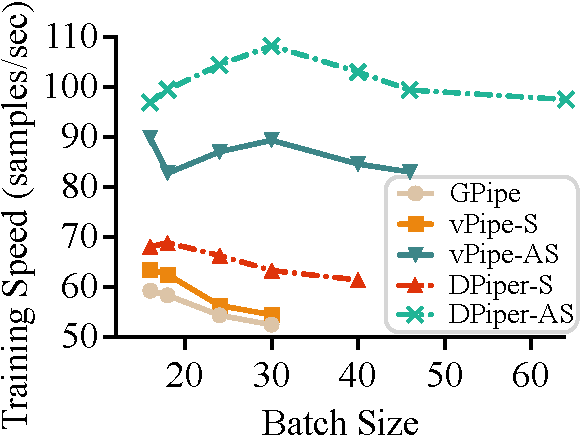
\includegraphics[width=0.47\linewidth]{BERT-4GPU-crop.pdf}
  }
  \subfigure[GPT-2]{
    \centering
    \label{subfig:gpt-2-4}
    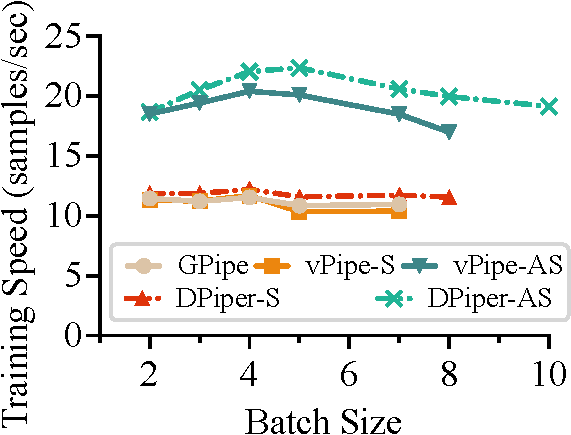
\includegraphics[width=0.47\linewidth]{GPT-2-4GPU-crop.pdf}
  }
  \subfigure[T5]{
    \centering
    \label{subfig:t5-4}
    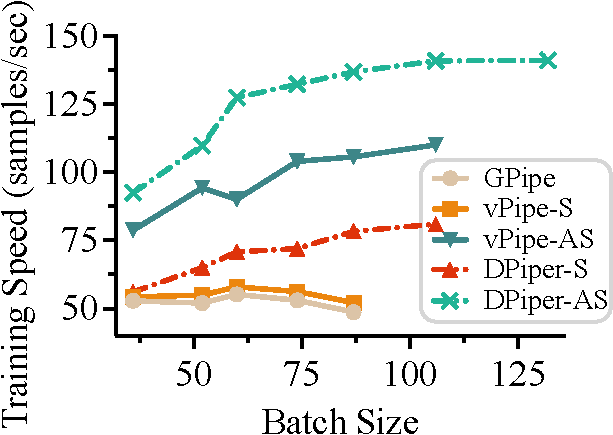
\includegraphics[width=0.47\linewidth]{T5-4GPU-crop.pdf}
  }
  \subfigure[AmoebaNet]{
    \centering
    \label{subfig:amoebanet-4}
    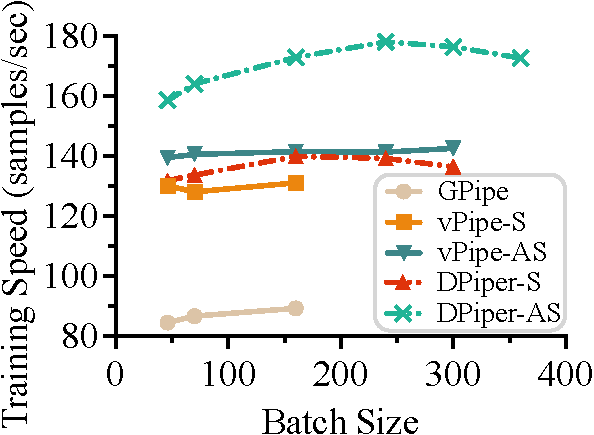
\includegraphics[width=0.47\linewidth]{AmoebaNet-4GPU-crop.pdf}
  }
  \caption{Training Speed under Pipeline Stage of 4}
  \label{fig:perf-4}
\end{figure}
% because except for a more obvious difference in the model division on AmoebaNet,
% the differences on the other three models are relatively small.

% This is because in the experiments of this chapter, the number of micro-batches executed simultaneously
% in the first stage of both synchronous and asynchronous pipeline parallelism is consistent,
% so an effective comparison can be made. 

% It should be noted that since the ZeRO and PipeDream methods
% do not perform memory optimization operations,
% they can only run at the initial batch size before memory overflow,
% so they are excluded for comparison.
% However, a brief explanation of the training performance of the ZeRO method is that as the model scale increases,
% the data parallelism will start to show a significant performance decline compared to pipeline parallelism
% due to the large amount of communication.
% For example, ZeRO's training speed on the relatively small BERT model is 1.4$\times$ that of GPipe at a smaller batch size,
% but on the larger GPT-2 model, the training speed drops to only 20\% of GPipe.
% As for PipeDream, its performance at the trainable batch size can refer to vPipe-AS,
% because except for a more obvious difference in the model division on AmoebaNet,
% the differences on the other three models are relatively small.

The training speed comparison results when pipeline stage is 4 is shown as Figure~\ref{fig:perf-4}.
% For the case of a pipeline stage number of 4,
% the training speed comparison of each method on the 4 models is shown in Figure~\ref{fig:perf-4}.
The training performance of synchronous pipeline parallelism
is significantly lower than that of the asynchronous pipeline parallelism
due to the pipeline bubbles caused by the computation synchronization.
% its training performance is significantly lower than that of asynchronous pipeline methods.
The performance of vPipe-S is generally better than GPipe,
and the advantage is more obvious on AmoebaNet,
because GPipe does not consider communication overhead between stages,
and an unreasonable partition on CNN models is more
likely to cause larger communication volumes,
while both DawnPiper and vPipe have considered the communication overhead in pipeline partition.

At a small batch size, DawnPiper does not have a particularly large advantage over other methods,
with an average performance improvement of about 7\%, and only a 17\% and 14\% performance improvement
in the asynchronous training mode on the T5 and AmoebaNet models, respectively.
Because DawnPiper can only rely on a more refined pipeline partition space
to find a better model partition when the memory is not oversubscribed.
As the batch size increases, other methods need to
perform memory optimization to meet the memory requirements for model training.
DawnPiper has a noticeable stage of increased training speed compared to other methods.
This improvement results from two folds, on the one hand,
the GPU compute resources can be better utilized when the batch size increases.
On the other hand, DawnPiper can:
a) adjust the memory footprint of each stage with minimal impact on the computation time;
b) reduce the memory footprint with almost no performance overhead by memory swapping
when the batch size is relatively small.
The first point can be achieved due to the observation on the memory usage
characteristics during training which is described in Section~\ref{sec:mot}.
% because it can make more full use of GPU resources when the batch increases from small to large,
% and on the other hand, it is also because DawnPiper can: 1) Change the memory occupation between pipeline stages
% with minimal impact on the computation of the pipeline stages;
% 2) Reduce memory occupation with almost no performance overhead by memory swapping when the batch is small.
Therefore, in synchronous pipeline parallelism,
DawnPiper achieved up to 1.5$\times$ performance improvement
on the T5 model when the batch size increased,
and up to 1.41$\times$ in the asynchronous mode.
Overall, as the batch size increases,
DawnPiper has an average performance improvement of 1.2$\times$, 1.12$\times$,
1.32$\times$, and 1.24$\times$ over vPipe in the asynchronous parallel training
on BERT, GPT-2, T5, and AmoebaNet, respectively.

The evaluations are only performed on GPT-2 and T5 as the pipeline stages increases to 8,
since the model sizes of BERT and AmoebaNet are too small for 8 GPUs.
The results are shown as Figure~\ref{fig:perf-8}.
% When the number of pipeline stages increases to 8,
% the evaluations on BERT and AmoebaNet are excluded
% since their model size is too small for 8 GPUs.
% The training speed results of GPT-2 and T5 are shown as Figure~\ref{fig:perf-8}.
% due to the size of the BERT model and the AmoebaNet model being too small relative to 8 GPUs,
% resulting in a relatively small amount of computation after division for each stage,
% this section only tests the GPT-2 model and the T5 model on 8 GPUs, which is shown as Figure~\ref{fig:perf-8}.
In the synchronous mode, the performance of GPT-2 on DawnPiper, GPipe, and vPipe is quite similar.
This is because the balanced partition positions of computation and memory for GPT-2
are very close, thus the partition optimization space is very limited.
% For the GPT-2 model, in the synchronous pipeline mode, the performance of DawnPiper, GPipe, and vPipe
% is quite close because their balanced division of computation and memory is very similar,
% thus the space for optimization is very limited.
In the asynchronous mode,
as the batch size gradually increases,
DawnPiper's training speed is by average 1.15$\times$ and 1.34$\times$
faster than vPipe on GPT-2 and T5, respectively.
DawnPiper has a better performance improvement on T5
due to its mixed model architecture based on encoder and decoder,
which has a more complex structure for providing partition space for DawnPiper.
% The T5 model, due to its being a Transformer model with a mix of encoder and decoder,
% has a more complex structure, providing more division space for DawnPiper,
% hence DawnPiper's performance improvement over vPipe is also greater.
Moreover, when the pipeline stages increase to 8,
DawnPiper also demonstrates good scalability.

\begin{figure}[htb]
  \centering
  % \hspace{-0.7cm}
  \subfigure[GPT-2]{
    \centering
    \label{subfig:gpt-2-8}
    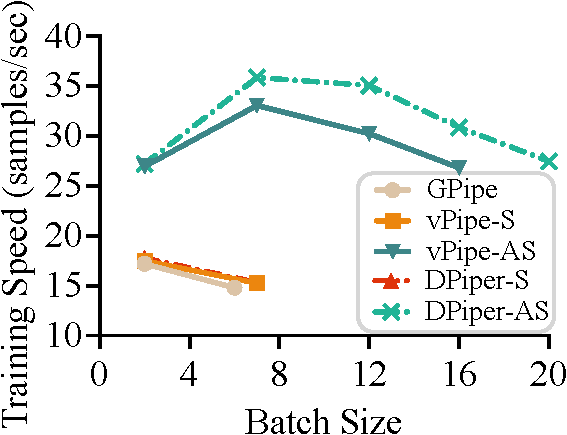
\includegraphics[width=0.47\linewidth]{GPT-2-8GPU-crop.pdf}
  }
  \subfigure[T5]{
    \centering
    \label{subfig:t5-8}
    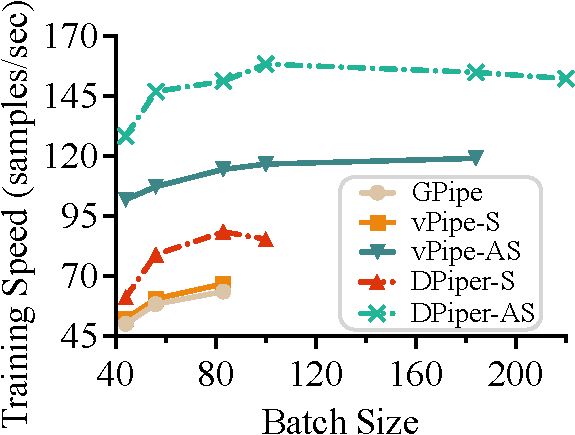
\includegraphics[width=0.47\linewidth]{T5-8GPU-crop.pdf}
  }
  \caption{Training Speed under Pipeline Stage of 8}
  \label{fig:perf-8}
\end{figure}

\subsection{Detailed analysis on computation time and memory footprint}
To provide a more detailed comparison on the memory footprint and computation of DawnPiper and vPipe,
we profile the GPU peak memory usage and computaiton time
of each stage on T5 in asynchronous mode under the pipeline stage of 8.
The micro-batch size is 110 which exceeds the maximum batch size that vPipe
can achieve without memory optimization by 2.5$\times$.
The results are shown in Figure~\ref{fig:mem-comp}. 
% this section selects the GPU memory usage and computation time
% of each stage after the division of the T5 model by vPipe and DawnPiper
% when the asynchronous pipeline stage number is 8,
% with a micro-batch size of 110, which exceeds the maximum batch size that vPipe
% can achieve without memory optimization by 2.5$\times$.
% The results are shown in Figure~\ref{fig:mem-comp}. 

Firstly, regarding to the peak memory usage of each stage,
it can be seen that DawnPiper occupies more GPU memory than vPipe
and the memory usage of each stage is more balanced.
This is because vPipe performs a coarser-grained pipeline partition and memory optimization,
while DawnPiper perform finer-grained memory optimization
to meet the memory requirements of each stage.
The overall GPU memory utilization is improved by 17.8\% compared to vPipe. 
In the meantime, the computation time of each stage under
DawnPiper's partition strategy also becomes more balanced,
with the difference between the longest and shortest execution time stages being only 7.7\%.
This ratio reaches 35.8\% under the vPipe's partition and memory optimization strategy

\begin{figure}
  \centering
  \includegraphics*[width=0.8\linewidth]{mem-comp.pdf}
  \caption{Peak Memory Usage and Computation time Analysis}
  \label{fig:mem-comp}
\end{figure}


% %!TEX root = main.tex
\section{Discussion}
% \paragraph{Distributed Training}
\setlength{\parindent}{2em}\textbf{\textit{a) Distributed training:}}
Distributed training is common to speedup the overall training process
and support massive models, such as GPT-serial models~\cite{radford2019language,brown2020language}.
It includes data parallelism, model parallelism~\cite{shoeybi2019megatron}, and pipeline model parallelism~\cite{ghuangGpipeEfficientTraining2019,narayanan2019pipedream,eliad2021fine}.
% But the is much difficult compared to singe-GPU training.
The distributed training is complicated than single-GPU training
as it introduces communication and parameters aggregation across GPUs.
Nonetheless, the memory usage of an iteration inside a single GPU still follows \emph{``first increase then drop"} pattern.
Therefore, the idea in \oursys{} is still applicable in distributed training.
% The concurrent training on distributed training ,
But the selection of jobs to co-locate with distributed training job needs to be more careful,
since the speed slowdown on one GPU lead to the performance degradation of overall distributed training.
% one slowdown on a GPU will 
We leave the extension of \oursys{} to distributed training as a future work.

\textbf{\textit{b) Job priority:}}
% \paragraph{Job priority}
There are usually two kinds of jobs in DL GPU cluster: \emph{high-priority job} and \emph{low-priority job}.
When co-locating jobs with different priorities,
it's an important and challenging problem to provide performance guarantee on jobs with high-priority.
AntMan~\cite{xiao2020antman} made an attempt to achieve it through limiting the operator launch rate of low-priority jobs.
The current scheduling in \oursys{} does not take the job priority into account.
Nonetheless, it's easy to integrate the batch scheduling policy or operator scheduling policy into \oursys{} to achieve prioritized scheduling,
since all jobs' batches are submitted to \oursys{} and the operator scheduling can also be achieved via NodeGroup abstract in \oursys{}.
And it's an interesting topic that how to achieve memory sharing efficiency while guaranteeing the job priority.
We leave the consideration of job priority and computation time as a future work.

\textbf{\textit{c) Balancing computation in graph partition and scheduling:}}
% \paragraph{Computation time consideration in graph partition and scheduling}
In graph partition and scheduling of \oursys{},
we only consider balancing the memory footprint of each partition without considering the balance of computation.
In general, when both jobs have high GPU computation demand and can fully utilize the GPU,
imbalanced computation of node groups will have little impact on performance.
However, if one of the models has lower computational demands,
imbalanced computation will degrade the performance to some extent.
However, a significant challenge in taking the computation demand into account is that
parallel kernel scheduling in NVIDIA GPU is opaque.
Therefore, it is difficult to predict whether the kernels in question can be parallelized and assess the performance of parallelized kernels.
As a result, it is challenging to determine if a particular partition and scheduling policy can achieve higher training throughput.
Novel methods need to be developed to overcome these difficulties, which is part of our future research plan.
% A major obstacle to take computation time into account
% is that the parallel kernels scheduling in NVIDIA GPU is a black box concurrently,
% which means it's difficult to predict whether the specific kernels can be parallelized executing
% or the performance of the parallelized kernels.
% Therefore, it's hard to judge if a specific partition and scheduling policy could
% achieve the best overall training throughput.

\textbf{\textit{d) Security:}}
% \paragraph{Security}
Security is crucial for DL training as this process could last long for months,
an accident exiting due to unpredictable faults will waste expensive GPU resources.
When jobs are running in their own CUDA context on the same GPU,
the fault only affects themselves, not to other jobs.
However, in order to share the GPU memory resources across jobs,
they need to run in the same CUDA context,
which will break the \emph{fault isolation}:
% one jobs's fault will lead all other co-located jobs exiting accidentally too.
the failure in a job doesn't impact other co-located jobs.
This security issue exists in the frameworks that merge numerous jobs' contexts into one,
such as NVIDIA MPS~\cite{mps}, Salus~\cite{yu2020salus}, and also \oursys{}.
A good aspect is that DL training job can be recovered at an arbitrary step
as long as the training state (parameters) at that step has been saved.
And this recovery is lightweight since the time to run a single training step is small (seconds level).
But too frequent checkpointing will also influence the overall training performance.
The users need to balance the frequency of checkpointing to make a tradeoff.
% Our work's priority purpose is to improve memory sharing efficiency in concurrent training
% Since share , the concurrent training jobs need to in the same CUDA context
% One job's fault will lead other co-located jobs fail too.
On the other side, another method to support concurrent running of multiple jobs
while guaranteeing fault isolation is virtualizing a GPU to numerous virtualized GPUs (vGPU)~\cite{vGPU}.
The latest technology is Multi-Instance GPU (MIG)~\cite{mig} which is provided by NVIDIA
and supported on the NVIDIA Ampere architecture and after (such as A100 and H100 GPU).
MIG partitions a single GPU into numerous separate GPU instances
where each one owns the dedicated compute, memory, and memory bandwidth resources.
But it has limitations for supporting concurrent training.
First, the compute and memory resource configurations of a GPU instance are pre-defined by NVIDIA that cannot be changed at will.
Besides, when the GPU instances have been configured, the resources cannot be adjusted flexible on-fly.
This collides with the diverse and dynamic resources requirement of DL training jobs.
% The DL training jobs' resource requirements vary much.
Second, the GPU memory resources are isolated across instances, thus cannot be shared.
% It's more suitable for AI inference tasks whose .
% But the optional configurations are limited.
% The compute and memory resources can not be adjusted flexible when the virtualized has been configured.
% \paragraph{Memory fragmentation}
% The next batch of a job won’t start until current batch has finished due to batch dependency.
% Therefore, all memory will be freed and coalesced to a large chunk naturally
% when current parallel running batches complete if there are only two jobs.
% When there are more than two jobs, we flush the pipeline when the parallel running
% batches of these jobs complete to avoid memory fragmentation.
% The memory fragmentation in concurrent training is an interesting topic to research.

%!TEX root = main.tex
\section{Related Work}
\label{sec:related}
\subsection{Data Parallelism}
Data parallelism is the most widely used parallel strategy which
divides the training data into multiple shards and distribute them to different devices.
As the model parameters and optimizer states gradually
accounts for a significant portion of the memory in NLP models training,
Ren et al. proposed the Zero Redundancy Optimizer (ZeRO)~\cite{rajbhandariZeROMemoryOptimizations2020}
to distribute such memory to store evenly in different devices.
ZeRO-Offload~\cite{renZerooffloadDemocratizingBillionScale2021} offloads all parameters and computations of the optimizer
to the CPU and redesigns the CPU optimizer computation method to accelerate this process.
ZeRO-Infinity~\cite{rajbhandariZeROinfinityBreakingGPU2021} further utilizes the memory optimization of offloading
the optimizer to the CPU in ZeRO-Offload
and the memory exchange method of offloading GPU memory to the CPU,
non-volatile memory (Non-Volatile Memory, NVM),
and other external storage to expand GPU memory.
PatrickStar~\cite{fangParallelTrainingPreTrained2022} proposed organizing memory in blocks and
using it as the communication unit for improving
the communication bandwidth utilization.
Generally, the data parallelism is orthogonal to our work
which can be used for training model in conjunction.

\subsection{Pipeline and Hybrid Parallelism}
GPipe~\cite{huangGpipeEfficientTraining2019} and PipeDream~\cite{narayananPipeDreamGeneralizedPipeline2019} are the pioneer work of
the SPP and ASP.
DAPPLE~\cite{fanDAPPLEPipelinedData2021} introduces the 1F1B computation scheduling into SPP by dividing the batch into
more micro-batches for the initial warm-up phase of computation scheduling.
It reduces the pipeline bubbles at the cost that relying on a sufficient number of micro-batches,
which is not always the case for NLP models.
Chimera~\cite{liChimeraEfficientlyTraining2021} proposes a bidirectional synchronous pipeline scheduling method,
which reduces the pipeline bubbles by letting a GPU perform the
forward and backward computations of two different stages.
Hanayo~\cite{liuHanayoHarnessingWavelike2023} combines the methods of DAPPLE and Chimera,
proposing a wave-based computation scheduling method.
Narayanan et al.~\cite{narayananEfficientLargeScaleLanguage2021} reduce the proportion of pipeline bubbles
by allowing a stage's GPU to store more model partitions
based on DAPPLE's computation scheduling, but at the cost of more communications.
Qi et al.~\cite{qiZeroBubbleAlmost} achieves almost bubble-free pipeline parallelism by
re-scheduling the backward computation.
% into two parts:
% computing gradients for inputs and computing gradients for model parameters,
% the idea being that there is no computational dependency
% for the part that computes gradients for model parameters,
% but to fully achieve no pipeline bubbles will result in more memory occupation.
BPipe~\cite{kimBPipeMemoryBalancedPipeline2023} balances the GPU memory usage between stages
by asynchronously exchanging activations between GPUs.
vPipe~\cite{zhaoVPipeVirtualizedAcceleration2022} proposes an iterative algorithm to dynamically find a balance between
model partitioning, memory swapping, and recomputation,
using the Kernighan-Lin algorithm~\cite{kernighanEfficientHeuristicProcedure1970}.
AdaPipe~\cite{sunAdaPipeOptimizingPipeline2024} proposes a two-step dynamic programming pipeline partition
and recomputation algorithm for SPP.
The pipeline parallelism is usually adopted in conjunction with tensor parallelism,
such as Flexflow~\cite{jiaDataModelParallelism2019} and Alpa~\cite{zhengAlpaAutomatingInter2022}, which is called as \emph{hybrid parallelism}.
We leave the extension for hybrid parallelism of DawnPiper to the future work.

% \subsection{Memory Optimization in Training}

%

%!TEX root = main.tex
% \section{Conclusions and Future Works}
\section{Conclusions}
\label{sec:conclusion}
This paper proposes a memory scablable pipeline parallel training framework named DawnPiper,
which aims at achieving efficient pipeline parallel training while reducing the waste of GPU memory resources,
thereby supporting the pipeline parallel training of larger-scale models under limited GPU resources.
DawnPiper first compiles and profiles the model to obtain its fine-grained computation graph and computation memory usage characteristics,
refining the model partitioning and memory optimization space.
Then, based on the observation of the model's memory usage characteristics during the training process,
it designs a binary pipeline parallel partitioning method based on partition range limitation,
combined with a memory optimization method based on the cost model, greatly reducing the search space of pipeline parallel partitioning.
The experimental results on four typical DNNs show that DawnPiper can increase the trainable batch size by an average of
1.29 times and 1.71 times compared to GPipe and vPipe, respectively, and can even reach 4.8-11 times compared to PipeDream,
and can accelerate the parallel training speed of vPipe by up to 1.5 times.

%
%!TEX root = main.tex
\section*{Acknowledgments}
This work was supported in part by the National Key R\&D Program of China under Grant 2020AAA0108501, and the Key R\&D Program of Hubei under Grant 2020BAA020.

%%%%%%%%%%%%%%%%%%%%%%%%%%%%%%%%%%%%%%%%%%%%%%%%%%%%%%%%%%%%%%%%%%%%%%%%%%%


{\footnotesize 
\bibliographystyle{IEEEtran}
\bibliography{./bib/papers}
}

% \vspace{-1cm}
% \begin{IEEEbiography}[{\includegraphics[width=1in,height=1.25in,clip,keepaspectratio]{XuanhuaShi-E.jpg}}]{Xuanhua Shi}
% (Senior Member, IEEE) received the PhD degree in computer engineering from the Huazhong University of Science and Technology, Wuhan, China, in 2005. He is currently a professor with the National Engineering Research Center for Big Data Technology and System Services Computing Technology and System/Services Computing Technology and System Lab, Huazhong University of Science and Technology (China). From 2006, he worked as an INRIA postdoctoral in PARIS team at Rennes for one year. His research interests cloud computing and big data processing. He published over more than 100 peer-reviewed publications, received research support from a variety of governmental and industrial organizations, such as National Science Foundation of China, Ministry of Science and Technology, Ministry of Education, European Union, Alibaba, ByteDance, Intel and so on. He is a senior member of CCF.
% \end{IEEEbiography}
% \vspace{-0.8cm}
% \begin{IEEEbiography}[{\includegraphics[width=1in,height=1.25in,clip,keepaspectratio]{xuan-2inch-E.jpg}}]{Xuan Peng}
% is currently working toward the PhD degree with the School of Computer Science and Technology, Huazhong University of Science and Technology, Wuhan, China. His research focuses on intelligent computing, memory management for AI systems.
% \end{IEEEbiography}
% \vspace{-0.8cm}
% \begin{IEEEbiography}[{\includegraphics[width=1in,height=1.25in,clip,keepaspectratio]{LigangHe.jpg}}]{Ligang He}
%   is now a Reader in the Department of Computer Science at the University of Warwick, UK. His research area is mainly parallel and distributed computing. He has published more than 150 papers in the research area.
% \end{IEEEbiography}
% \vspace{-0.5cm}

% \begin{IEEEbiography}[{\includegraphics[width=1in,height=1.25in,clip,keepaspectratio]{HaiJin-E.jpg}}]{Hai Jin}
% (Fellow, IEEE) received the Ph.D. degree in computer engineering from the Huazhong University of Science and Technology in 1994. He received the German Academic Exchange Service Fellowship to visit the Technical University of Chemnitz, Germany, in 1996. He worked at The University of Hong Kong from 1998 to 2000 and as a Visiting Scholar at the University of Southern California from 1999 to 2000. He received the Excellent Youth Award from the National Science Foundation of China in 2001. He is a Cheung Kung Scholars Chair Professor of computer science and engineering of the Huazhong University of Science and Technology. He has coauthored 22 books and published over 800 research articles. His research interests include computer architecture, virtualization technology, cluster computing and cloud computing, peer-to-peer computing, network storage, and network security. He is a fellow of the CCF and a member of the ACM.
% \end{IEEEbiography}

\end{document}